%%
%% Copyright 2007-2024 Elsevier Ltd
%%
%% This file is part of the 'Elsarticle Bundle'.
%% ---------------------------------------------
%%
%% It may be distributed under the conditions of the LaTeX Project Public
%% License, either version 1.3 of this license or (at your option) any
%% later version.  The latest version of this license is in
%%    http://www.latex-project.org/lppl.txt
%% and version 1.3 or later is part of all distributions of LaTeX
%% version 1999/12/01 or later.
%%
%% The list of all files belonging to the 'Elsarticle Bundle' is
%% given in the file `manifest.txt'.
%%
%% Template article for Elsevier's document class `elsarticle'
%% with harvard style bibliographic references

\documentclass[preprint,12pt,authoryear]{elsarticle}

%% Use the option review to obtain double line spacing
%% \documentclass[authoryear,preprint,review,12pt]{elsarticle}

%% Use the options 1p,twocolumn; 3p; 3p,twocolumn; 5p; or 5p,twocolumn
%% for a journal layout:
%% \documentclass[final,1p,times,authoryear]{elsarticle}
%% \documentclass[final,1p,times,twocolumn,authoryear]{elsarticle}
%% \documentclass[final,3p,times,authoryear]{elsarticle}
%% \documentclass[final,3p,times,twocolumn,authoryear]{elsarticle}
%% \documentclass[final,5p,times,authoryear]{elsarticle}
%% \documentclass[final,5p,times,twocolumn,authoryear]{elsarticle}

%% For including figures, graphicx.sty has been loaded in
%% elsarticle.cls. If you prefer to use the old commands
%% please give \usepackage{epsfig}

%% The amssymb package provides various useful mathematical symbols
\usepackage{amssymb}
%% The amsmath package provides various useful equation environments.
\usepackage{amsmath}
%% The amsthm package provides extended theorem environments
%% \usepackage{amsthm}

%% The lineno packages adds line numbers. Start line numbering with
%% \begin{linenumbers}, end it with \end{linenumbers}. Or switch it on
%% for the whole article with \linenumbers.
%% \usepackage{lineno}

%% The booktabs package provides table makeup macros.
\usepackage{booktabs}

%% Custom math operators
\DeclareMathOperator*{\argmax}{argmax}
\DeclareMathOperator*{\argmin}{argmin}
\DeclareMathOperator{\sgn}{sgn}

\journal{Computational Statistics and Data Analysis}

\begin{document}

\begin{frontmatter}

%% Title, authors and addresses

%% use the tnoteref command within \title for footnotes;
%% use the tnotetext command for theassociated footnote;
%% use the fnref command within \author or \affiliation for footnotes;
%% use the fntext command for theassociated footnote;
%% use the corref command within \author for corresponding author footnotes;
%% use the cortext command for theassociated footnote;
%% use the ead command for the email address,
%% and the form \ead[url] for the home page:
%% \title{Title\tnoteref{label1}}
%% \tnotetext[label1]{}
%% \author{Name\corref{cor1}\fnref{label2}}
%% \ead{email address}
%% \ead[url]{home page}
%% \fntext[label2]{}
%% \cortext[cor1]{}
%% \affiliation{organization={},
%%            addressline={},
%%            city={},
%%            postcode={},
%%            state={},
%%            country={}}
%% \fntext[label3]{}

\title{Location and Scale-Invariant Power Transformations for Transforming Data to Normality} %% Article title

%% use optional labels to link authors explicitly to addresses:
%% \author[label1,label2]{}
%% \affiliation[label1]{organization={},
%%             addressline={},
%%             city={},
%%             postcode={},
%%             state={},
%%             country={}}
%%
%% \affiliation[label2]{organization={},
%%             addressline={},
%%             city={},
%%             postcode={},
%%             state={},
%%             country={}}


%% Alex Zwanenburg
\author[affil_1,affil_2]{Alex Zwanenburg\corref{cor_note}}
\ead{alexander.zwanenburg@nct-dresden.de}
\cortext[cor_note]{corresponding author}

\affiliation[affil_1]{
  organization={
    National Center for Tumor Diseases Dresden (NCT/UCC):
    German Cancer Research Center (DKFZ), Heidelberg, Germany;
    Faculty of Medicine and University Hospital Carl Gustav Carus, TUD Dresden University of Technology, Dresden, Germany;
    Helmholtz-Zentrum Dresden-Rossendorf (HZDR), Dresden, Germany},
  addressline={Fetscherstraße 74/PF 64},
  city={Dresden},
  postcode={01307},
  country={Germany}
}
\affiliation[affil_2]{
  organization={
    OncoRay – National Center for Radiation Research in Oncology,
    Faculty of Medicine and University Hospital Carl Gustav Carus, TUD Dresden University of Technology,
    Helmholtz-Zentrum Dresden-Rossendorf},
  addressline={Fetscherstraße 74/PF 41},
  city={Dresden},
  postcode={01307},
  country={Germany}
}

%% Steffen Löck
\author[affil_2,affil_3,affil_4]{Steffen Löck}

\affiliation[affil_3]{
  organization={
    Department of Radiotherapy and Radiation Oncology,
    Faculty of Medicine and University Hospital Carl Gustav Carus, TUD Dresden University of Technology},
  addressline={Fetscherstraße 74/PF 50},
  city={Dresden},
  postcode={01307},
  country={Germany}
}
\affiliation[affil_4]{
  organization={
   German Cancer Consortium (DKTK), Partner Site Dresden,
   and German Cancer Research Center (DKFZ)},
  addressline={Im Neuenheimer Feld 280},
  city={Heidelberg},
  postcode={69192},
  country={Germany}
}



%% Abstract
% You are required to provide a concise and factual abstract which does not exceed
% 250 words. The abstract should briefly state the purpose of your research,
% principal results and major conclusions. Some guidelines:
%
% Abstracts must be able to stand alone as abstracts are often presented separately from the article.
%
% Avoid references. If any are essential to include, ensure that you cite the author(s) and year(s).
%
% Avoid non-standard or uncommon abbreviations. If any are essential to include,
% ensure they are defined within your abstract at first mention.

\begin{abstract}
Power transformations are used to stabilize variance and achieve
normality of features, especially in methods assuming normal 
distributions such as ANOVA and linear discriminant analysis. 
However, the commonly used Box-Cox and Yeo-Johnson power transformation 
methods are sensitive to the location, scale, and presence of 
outliers in the data.

Here we present location- and scale-invariant Box-Cox and Yeo-Johnson
transformations to mitigate these issues. We derive maximum likelihood
estimation criteria for optimizing transformation parameters and propose
robust adaptations that reduce the influence of outliers. 
We also introduce an empirical test for assessing central normality
of transformed features.

In simulations and real-world datasets, robust location- and scale-invariant 
transformations outperform conventional variants, resulting in better 
transformations to central normality. In a machine learning experiment
with 232 datasets with numerical features, integrating robust 
ocation- and scale-invariant power transformations into an automated data 
processing and machine learning pipeline did not result in a meaningful
improvement or detriment in model performance compared to conventional variants.

In conclusion, robust location- and scale-invariant power
transformations can replace conventional variants.
\end{abstract}

%%Graphical abstract
% \begin{graphicalabstract}
% \includegraphics{grabs}
% \end{graphicalabstract}

%%Research highlights
% Highlights are a short collection of bullet points that should capture the novel
% results of your research as well as any new methods used during your study.
% Highlights will help increase the discoverability of your article via search engines.
% Some guidelines:
%
% Submit highlights as a separate editable file in the online submission system
% with the word "highlights" included in the file name.
%
% Highlights should consist of 3 to 5 bullet points, each a maximum of 85 characters, including spaces.

\begin{highlights}
\item Location and scale of feature distributions may cause wrong power transformations.
\item We derived location- and scale-invariant Box-Cox and Yeo-Johnson transformations.
\item Robust power transformations succesfully reduced negative effects of outliers.
\item New invariant robust power transformations can replace conventional variants.
\end{highlights}

%% Keywords
% You are required to provide 1 to 7 keywords for indexing purposes. Keywords should be written in English.
% Please try to avoid keywords consisting of multiple words (using "and" or "of").
% We recommend that you only use abbreviations in keywords if they are firmly established in the field.
\begin{keyword}

power transformation \sep invariant transformation \sep robust transformation \sep normality test
%% keywords here, in the form: keyword \sep keyword

%% PACS codes here, in the form: \PACS code \sep code

%% MSC codes here, in the form: \MSC code \sep code
%% or \MSC[2008] code \sep code (2000 is the default)

\end{keyword}

\end{frontmatter}

%% Add \usepackage{lineno} before \begin{document} and uncomment
%% following line to enable line numbers
%% \linenumbers

%% main text
%%
\section{Introduction}\label{introduction}

Many statistical and some machine learning methods assume normality of
the underlying data, e.g.~analysis of variance and linear discriminant
analysis. However, numerical features in datasets may strongly deviate
from normal distributions, e.g.~by being skewed. Power transformations
aim to stabilise variance and improve normality of such features
\citep{Bartlett1947-rx, Tukey1957-rt}. The two most commonly used
transformations are that of \citet{Box1964-mz} and \citet{Yeo2000-vw}.
The Box-Cox transformation of a feature value \(x_i\) of feature
\(\mathbf{X}=\left\{x_1, x_2, \ldots, x_n \right\}\) under the
transformation parameter \(\lambda\) is defined as:

\begin{equation}
\label{eqn:box-cox-original}
\phi_{\text{BC}}^\lambda (x_i) = 
\begin{cases}
\left(x_i^\lambda - 1 \right) / \lambda & \text{if } \lambda \neq 0\\
\log(x_i) & \text{if } \lambda = 0
\end{cases}
\end{equation}

One limitation of the Box-Cox transformation is that it is only defined
for \(x_i > 0\). In contrast, the Yeo-Johnson transformation under the
transformation parameter \(\lambda\) is defined for any
\(x_i \in \mathbb{R}\):

\begin{equation}
\label{eqn:yeo-johnson-original}
\phi_{\text{YJ}}^\lambda (x_i) = 
\begin{cases}
\left( \left( 1 + x_i \right)^\lambda - 1\right) / \lambda & \text{if } \lambda \neq 0 \text{ and } x_i \geq 0\\
\log(1 + x_i) & \text{if } \lambda = 0 \text{ and } x_i \geq 0\\
-\left( \left( 1 - x_i\right)^{2 - \lambda} - 1 \right) / \left(2 - \lambda \right) & \text{if } \lambda \neq 2 \text{ and } x_i < 0\\
-\log(1 - x_i) & \text{if } \lambda = 2 \text{ and } x_i < 0
\end{cases}
\end{equation}

The \(\lambda\)-parameter is typically optimised using maximum
likelihood estimation under the assumption that the transformed feature
is normally distributed. As noted by Raymaekers and Rousseeuw, this
approach is sensitive to outliers, and robust versions of Box-Cox and
Yeo-Johnson transformations were devised \citep{Raymaekers2024-zf}.

Applying a power transformation does not guarantee that transformed
features are normally distributed. Depending on location and scale of a
feature and the presence of outliers, power transformations may decrease
normality, as shown in Figure \ref{fig:decreased-normality}. If
normality of the transformed feature is not checked, e.g.~in automated
power transformation in machine learning workflows, several issues may
arise. For example, statistical tests such as ANOVA may produce
incorrect results due to violation of the normality assumption.
Likewise, machine learning methods that assume normality of input
features may suffer a decrease in performance. Moreover, large negative
or positive \(\lambda\)-parameters may lead to numeric issues in any
subsequent computations.

Statistical tests for normality, such as the Shapiro-Wilk test
\citep{Shapiro1965-zd}, could be automatically applied to transformed features.
However, given sufficiently large sample sizes such tests can detect
trivial deviations from normality, and may lead to rejection of
sufficiently good power transformations.

\begin{figure}

{\centering 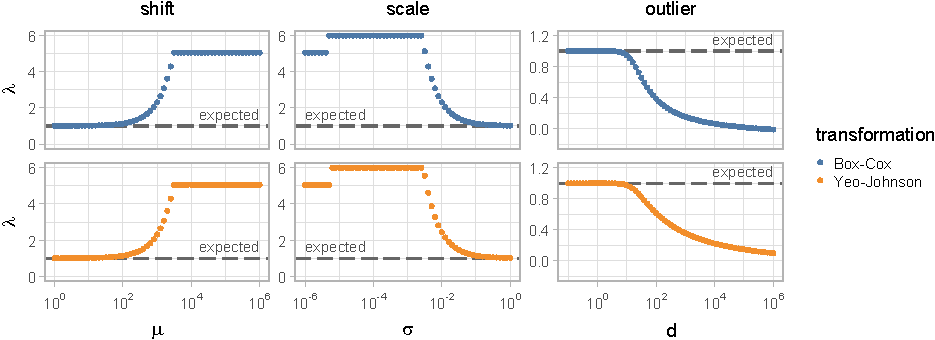
\includegraphics[width=1\linewidth]{figure_1} 

}

\caption{Effect of location, scale and outliers on estimation of the Box-Cox and Yeo-Johnson transformation parameter $\lambda$. $10000$ samples were drawn from a normal distribution: $\mathcal{N}(\mu, 1)$ for the shift dataset, $\mathcal{N}(10, \sigma)$ for the scale dataset and $\mathcal{N}(0, 1)$ for the outlier dataset. Additionally, an outlier with value $d$ was added to the outlier dataset. Since samples are drawn from a normal distribution, a transformation parameter of $\lambda = 1$ is expected. However, a large shift in location, a scale that is small compared to the location, or presence of large outliers lead to incorrectly estimated transformation parameter values.}\label{fig:decreased-normality}
\end{figure}

To address these issues, we make the following contributions:

\begin{itemize}
\item
  We devise location- and scale-invariant versions of the Box-Cox and
  Yeo-Johnson transformation, including versions robust to outliers.
\item
  We derive the maximum likelihood criterion for location- and
  scale-invariant Box-Cox and Yeo-Johnson transformations to allow for
  optimising transformation parameters.
\item
  We define an empirical central normality test for detecting cases
  where power transformations fail to yield an approximately normally
  distributed transformed feature.
\item
  We assess the effect of power transformations on the performance of
  machine learning models.
\end{itemize}

\section{Theory}\label{theory}

In this section, we will first introduce location- and scale-invariant
versions of the Box-Cox and Yeo-Johnson transformations. Subsequently,
we define weighted location- and scale-invariant transformations and
weighting methods for robust transformations. We then define the
quantile function for asymmetric generalised normal distributions to
enable random sampling. Finally, we define the overall framework for the
empirical central normality test.

\subsection{Location- and scale-invariant power
transformation}\label{location--and-scale-invariant-power-transformation}

Box-Cox and Yeo-Johnson transformations are modified by introducing
shift parameter \(x_0\) and scale parameter \(s\) into equations
\ref{eqn:box-cox-original} and \ref{eqn:yeo-johnson-original}. The
location- and scale-invariant Box-Cox transformation of a feature value
\(x_i\) of feature \(\mathbf{X}\) under transformation parameter
\(\lambda\), shift parameter \(x_0\) and scale parameter \(s\) is then:

\begin{equation}
\label{eqn:box-cox-invariant}
\phi_{\text{BC}}^{\lambda, x_0, s} (x_i) = 
\begin{cases}
\left( \left(\frac{x_i - x_0}{s} \right)^\lambda - 1 \right) / \lambda & \text{if } \lambda \neq 0\\
\log\left[\frac{x_i - x_0}{s}\right] & \text{if } \lambda = 0
\end{cases}
\end{equation}

where \(x_i - x_0 > 0\). Likewise, the location- and scale-invariant
Yeo-Johnson transformation of a feature value \(x_i\) under
transformation parameter \(\lambda\), shift parameter \(x_0\) and scale
parameter \(s\) is:

\begin{equation}
\label{eqn:yeo-johnson-invariant}
\phi_{\text{YJ}}^{\lambda, x_0, s} (x_i) = 
\begin{cases}
\left( \left( 1 + \frac{x_i - x_0}{s}\right)^\lambda - 1\right) / \lambda & \text{if } \lambda \neq 0 \text{ and } x_i - x_0 \geq 0\\
\log\left[1 + \frac{x_i - x_0}{s}\right] & \text{if } \lambda = 0 \text{ and } x_i - x_0 \geq 0\\
-\left( \left( 1 - \frac{x_i - x_0}{s}\right)^{2 - \lambda} - 1 \right) / \left(2 - \lambda \right) & \text{if } \lambda \neq 2 \text{ and } x_i - x_0 < 0\\
-\log\left[1 - \frac{x_i - x_0}{s}\right] & \text{if } \lambda = 2 \text{ and } x_i - x_0 < 0
\end{cases}
\end{equation}

For both invariant transformations, \(\lambda\), \(x_0\) and \(s\)
parameters can be obtained by maximising the log-likelihood function,
i.e.~using maximum likelihood estimation (MLE). A full derivation of the
log-likelihood function for both transformations is shown in \ref{appendix-a-log-likelihood-functions-for-location-and-scale-invariant-power-transformation}.
The location- and scale-invariant Box-Cox log-likelihood function is:

\begin{equation}
\label{eqn:box-cox-invariant-log-likelihood}
\begin{split}
\mathcal{l}_{\text{BC}}^{\lambda, x_0, s} = & -\frac{n}{2} \log \left[2 \pi \sigma^2 \right] -\frac{1}{2 \sigma^2} \sum_{i=1}^n \left( \phi_{BC}^{\lambda, x_0, s}(x_i) - \mu \right)^2 \\
& -n \lambda \log s + \left( \lambda - 1 \right) \sum_{i=1}^n \log \left[ x_i - x_0 \right]
\end{split}
\end{equation}

subject to \(x_i - x_0 > 0\). \(\mu\) and \(\sigma^2\) are the mean and
variance of the Box-Cox transformed feature
\(\phi_{\text{BC}}^{\lambda, x_0, s} (\mathbf{X})\), respectively.
Similarly, the location- and scale-invariant Yeo-Johnson log-likelihood
function is:

\begin{equation}
\label{eqn:yeo-johnson-invariant-log-likelihood}
\begin{split}
\mathcal{l}_{\text{YJ}}^{\lambda, x_0, s} = & -\frac{n}{2} \log\left[2 \pi \sigma^2\right] -\frac{1}{2 \sigma^2} \sum_{i=1}^n \left( \phi_{YJ}^{\lambda, x_0, s}(x_i) - \mu \right)^2 \\
& - n \log s + (\lambda - 1) \sum_{i=1}^n \sgn(x_i - x_0) \log \left[1 + \frac{|x_i - x_0|}{s} \right]
\end{split}
\end{equation}

where \(\mu\) and \(\sigma^2\) are the mean and variance of the
Yeo-Johnson transformed feature
\(\phi_{\text{YJ}}^{\lambda, x_0, s} (\mathbf{X})\), respectively.

\subsection{Robust location- and scale-invariant power
transformations}\label{robust-location--and-scale-invariant-power-transformations}

Real-world data may contain outliers, to which maximum likelihood
estimation can be sensitive. Their presence may lead to poor
transformations to normality, as shown in Figure
\ref{fig:decreased-normality}. As indicated by \citet{Raymaekers2024-zf},
the general aim of power transformations should be to transform
non-outlier data to normality, i.e.~achieve \emph{central normality}. To
achieve this, they devised an iterative procedure to find a robust
estimate of the transformation parameter \(\lambda\). Briefly, this
process requires identifying outliers in the data and weighting such
instances during the optimisation process. \citet{Raymaekers2024-zf}
achieve this through weighted maximum likelihood estimation.
However, because this procedure iteratively estimates and updates
\(\lambda\), it can not be used here to simultaneously estimate
\(\lambda\), \(x_0\) and \(s\) for location- and scale-invariant power
transformations. Nonetheless, as a procedure, weighted MLE can be used
for estimating the transformation, shift and scale parameters.

Here, weighted maximum likelihood estimation is based on equations
\ref{eqn:box-cox-invariant-log-likelihood} and
\ref{eqn:yeo-johnson-invariant-log-likelihood}. Compared to \citet{Raymaekers2024-zf},
these log-likelihood functions includes additional
terms to accommodate estimation of \(x_0\) and \(s\). The weighted
location- and scale-invariant Box-Cox log-likelihood function is:

\begin{equation}
\label{eqn:box-cox-weighted-invariant-log-likelihood}
\begin{split}
\mathcal{l}_{\text{rBC}}^{\lambda, x_0, s} = & -\frac{1}{2} \left(\sum_{i=1}^n w_i \right) \log \left[ 2 \pi \sigma_w^2 \right] -\frac{1}{2 \sigma_w^2} \sum_{i=1}^n w_i \left( \phi_{\text{BC}}^{\lambda, x_0, s}(x_i) - \mu_w \right)^2 \\
& - \lambda \left( \sum_{i=1}^n w_i \right) \log s + \left( \lambda - 1 \right) \sum_{i=1}^n w_i \log \left[ x_i - x_0 \right]
\end{split}
\end{equation}

where \(\mu_w\) and \(\sigma^2_w\) are the weighted mean and weighted
variance of the Box-Cox transformed feature
\(\phi_{\text{BC}}^{\lambda, x_0, s} (\mathbf{X})\):

\begin{equation}
\sigma_w^2 = \frac{\sum_{i=1}^n w_i \left(\phi_{\text{BC}}^{\lambda, x_0, s} (x_i) - \mu_w \right)^2}{\sum_{i=1}^n w_i} \quad \text{with } \mu_w = \frac{\sum_{i=1}^n w_i \phi_{\text{BC}}^{\lambda, x_0, s} (x_i)} {\sum_{i=1}^n w_i}
\end{equation}

Analogously, the weighted location- and scale-invariant Yeo-Johnson
log-likelihood function is:

\begin{equation}
\label{eqn:yeo-johnson-weighted-invariant-log-likelihood}
\begin{split}
\mathcal{l}_{\text{rYJ}}^{\lambda, x_0, s} = & -\frac{1}{2} \left(\sum_{i=1}^n w_i \right) \log \left[ 2 \pi \sigma_w^2 \right] -\frac{1}{2 \sigma_w^2} \sum_{i=1}^n w_i \left( \phi_{\text{YJ}}^{\lambda, x_0, s}(x_i) - \mu_w \right)^2 \\
& - \left( \sum_{i=1}^n w_i \right) \log s + (\lambda - 1) \sum_{i=1}^n w_i \sgn(x_i - x_0) \log \left[1 + \frac{|x_i - x_0|}{s} \right]
\end{split}
\end{equation}

where \(\mu_w\) and \(\sigma^2_w\) are the weighted mean and weighted
variance of the Yeo-Johnson transformed feature
\(\phi_{\text{YJ}}^{\lambda, x_0, s} (\mathbf{X})\):

\begin{equation}
\sigma_w^2 = \frac{\sum_{i=1}^n w_i \left(\phi_{\text{YJ}}^{\lambda, x_0, s} (x_i) - \mu_w \right)^2}{\sum_{i=1}^n w_i} \quad \text{with } \mu_w = \frac{\sum_{i=1}^n w_i \phi_{\text{YJ}}^{\lambda, x_0, s} (x_i)} {\sum_{i=1}^n w_i}
\end{equation}

The weights \(w_i\) in equations
\ref{eqn:box-cox-weighted-invariant-log-likelihood} and
\ref{eqn:yeo-johnson-weighted-invariant-log-likelihood} can be set using
several weighting functions. Using \(\dot{x}_i\) as an argument that
will be defined later, we investigate three weighting functions:

\begin{itemize}
\item
  A step function, with \(\delta_1 \geq 0\) as threshold parameter:
\end{itemize}

\begin{equation}
w_i =
\begin{cases}
1 & \text{if } \left| \dot{x}_i \right| \leq \delta_1\\
0 & \text{if } \left| \dot{x}_i \right| > \delta_1
\end{cases}
\end{equation}

\begin{itemize}
\item
  A triangle function (or generalised Huber weight), with
  \(\delta_1 \geq 0\) and \(\delta_2 \geq \delta_1\) as threshold
  parameters:
\end{itemize}

\begin{equation}
w_i =
\begin{cases}
1 & \text{if } \left| \dot{x}_i \right| < \delta_1\\
1 - \frac{\left| \dot{x}_i \right| - \delta_1}{\delta_2 - \delta_1} & \text{if } \delta_1 \leq \left| \dot{x}_i \right| \leq \delta_2 \\
0 & \text{if } \left| \dot{x}_i \right| > \delta_2
\end{cases}
\end{equation}

\begin{itemize}
\item
  A tapered cosine function \citep{Tukey1967-eb}, with \(\delta_1 \geq 0\)
  and \(\delta_2 \geq \delta_1\) as threshold parameters:
\end{itemize}

\begin{equation}
w_i =
\begin{cases}
1 & \text{if } \left| \dot{x}_i \right| < \delta_1\\
0.5 + 0.5 \cos\left(\pi \frac{\left| \dot{x}_i \right| - \delta_1}{\delta_2 - \delta_1} \right) & \text{if } \delta_1 \leq \left| \dot{x}_i \right| \leq \delta_2 \\
0 & \text{if } \left| \dot{x}_i \right| > \delta_2
\end{cases}
\end{equation}

All weighting functions share the characteristic that for
\(\left| \dot{x}_i \right|< \delta_1\), instances are fully weighted,
i.e.~when \(\delta_1 > 0\) the weighting functions are symmetric window
functions with a flat top. The triangle and tapered cosine functions
then gradually down-weight instances with
\(\delta_1 \leq \left| \dot{x}_i \right| \leq \delta_2\), and assign no
weight to instances \(\left| x_i \right| > \delta_2\). Examples of these
weighting function are shown in Figure \ref{fig:weighting-functions}.

\begin{figure}

{\centering 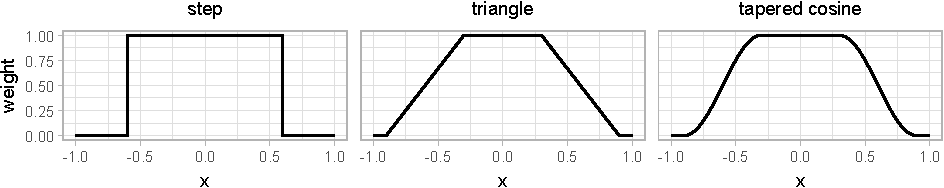
\includegraphics[width=1\linewidth]{figure_2} 

}

\caption{Weighting functions investigated in this study to make power transformations more robust against outliers. In this example, the step function was parameterised with $\delta_1 = 0.60$. The triangle and tapered cosine functions were both parameterised with $\delta_1 = 0.30$ and $\delta_2 = 0.90$.}\label{fig:weighting-functions}
\end{figure}

Each weighting function has an argument \(\dot{x}\) that is related to
the (transformed) feature in one of several ways:

\begin{itemize}
\item
  The weighting function uses empirical probabilities of the
  distribution of the original feature \(\mathbf{X}\). After sorting
  \(\mathbf{X}\) in ascending order, probabilities are determined as
  \(p_i = \frac{i - 1/3}{n + 1/3}\), with \(i = 1, 2, \ldots n\), with
  \(n\) the number of instances of feature \(\mathbf{X}\). Then
  \(\dot{x}_i = p^{*}_i=2 \left( p_i - 0.5\right)\), so that argument is
  zero-centered.
\item
  The weighting function uses the z-score of the transformed feature
  \(\phi^{\lambda, x_0, s} (\mathbf{X})\). After \citep{Raymaekers2024-zf},
  \(z_i = \frac{\phi^{\lambda, x_0, s}(x_i) - \mu_M}{\sigma_M}\). Here,
  \(\mu_M\) and \(\sigma_M\) are robust Huber M-estimates of location
  and scale of the transformed feature
  \(\phi^{\lambda, x_0, s} (\mathbf{X})\) \citep{Huber1981-su}. Then
  \(\dot{x}_i = z_i\).
\item
  After sorting \(\mathbf{X}\) in ascending order, the weighting
  function uses the residual error between the z-score of the
  transformed feature \(\phi^{\lambda, x_0, s} (\mathbf{X})\) and the
  theoretical z-score from a standard normal distribution:
  \(r_i =\left| \left( \phi^{\lambda, x_0, s}(x_i) - \mu_M)\right) / \sigma_M - F^{-1}_{\mathcal{N}}(p_i) \right|\),
  with \(\mu_M\), \(\sigma_M\) and \(p_i\) as defined above. Then
  \(\dot{x}_i = r_i\).
\end{itemize}

\subsection{Asymmetric generalised normal
distributions}\label{asymmetric-generalised-normal-distributions}

Modifications intended to make power transformations invariant to
location and scale of a feature and methods to improve their robustness
against outliers need to be assessed using data drawn from a range of
different distributions. Since the power transformations are intended
for use with unimodal distributions, the generalised normal distribution
\citep{Subbotin1923-qk, Nadarajah2005-xe} is a suitable option for simulating
realistic feature distributions. This distribution has the following
probability density function \(f_{\beta}\) for a value
\(x \in \mathbb{R}\):

\begin{equation}
f_{\beta}(x) = \frac{\beta}{2\Gamma\left(1 / \beta \right)} e^{-\left| x \right|^\beta}
\end{equation}

Here, \(\Gamma\) is the gamma function, and \(\beta\) is a strictly
positive shape parameter. For \(\beta = 1\), the probability density
function describes a Laplace distribution. A normal distribution is
found for \(\beta=2\), and for large \(\beta\), the distribution
approaches a uniform distribution. We will refrain from introducing
scale and location parameters here directly.

Realistic feature distributions may be skewed. Gijbels et al.~describe a
recipe for introducing skewness into the otherwise symmetric generalised
normal distribution \citep{Gijbels2019-te}, leading to
the following probability density function:

\begin{equation}
f_{\alpha}(x; \mu, \sigma, \beta) = \frac{2 \alpha \left(1 - \alpha\right)}{\sigma}
\begin{cases}
f_{\beta}\left( \left(1 - \alpha \right) \frac{\left| x - \mu \right|}{\sigma} \right) & \text{, } x \leq \mu \\
f_{\beta}\left( \alpha \frac{\left| x - \mu \right|}{\sigma} \right) & \text{, } x > \mu
\end{cases}
\end{equation}

Here, \(\alpha \in (0,1)\) is a skewness parameter. \(\alpha > 0.5\)
creates a distribution with a negative skew, i.e.~a left-skewed
distribution. A right-skewed distribution is created for
\(\alpha < 0.5\). \(\mu \in \mathcal{R}\) and \(\sigma \in (0, \infty)\)
are location and scale parameters, respectively. \(f_{\alpha}\) thus
describes the probability density function of an asymmetric generalised
normal distribution, which we will refer to here and parametrise as
\(\mathcal{AGN}\left(\mu, \sigma, \alpha, \beta \right)\).

We require a quantile function (or an approximation thereof) to draw
random values from an asymmetric generalised normal distribution using
inverse transform sampling. Gijbels et al.~derived the following
quantile function \(F_{\alpha}^{-1}(p)\):

\begin{equation}
F_{\alpha}^{-1}(p; \mu, \sigma, \beta) =
\begin{cases}
\mu + \frac{\sigma}{1 - \alpha} F_{\beta}^{-1} \left( \frac{p}{2 \alpha}\right) & \text{, } p \leq \alpha \\
\mu + \frac{\sigma}{\alpha} F_{\beta}^{-1} \left( \frac{1 + p - 2 \alpha}{2 \left(1 - \alpha \right)} \right) & \text{, } p > \alpha
\end{cases}
\end{equation}

The quantile function for the asymmetric generalised normal distribution
\(F_{\alpha}^{-1}\) thus incorporates the quantile function
\(F_{\beta}^{-1}\) of the symmetric generalised normal distribution.
\(F_{\beta}^{-1}\) was derived by Griffin to be \citep{Griffin2018-bf}:

\begin{equation}
F_{\beta}^{-1}(p) = \sgn\left(p - 0.5 \right) F_{\Gamma}^{-1}\left(2 \left|p - 0.5 \right|; 1 / \beta \right)
\end{equation}

Here, \(F_{\Gamma}^{-1}\) is the quantile function of the gamma
distribution with shape \(1 / \beta\), which can be numerically
approximated.

\subsection{Empirical central normality
test}\label{empirical-central-normality-test}

Power transformations aim to transform features to a normal
distribution. However, this may not always be successful or possible.
Deviations from normality can be detected by normality tests, such as
the Shapiro-Wilk test \citep{Shapiro1965-zd}. In practice, normality
tests may be too stringent with large sample sizes, outliers, or both.
Here we develop an empirical test for central normality. The null
hypothesis \(H_0\) is that the distribution is centrally normal. The
alternative hypothesis \(H_1\) is that the distribution is not centrally
normal.

Let central normality be defined as the normality of central portion
\(\kappa\) of the data,
i.e.~\(\mathbf{X}_{\text{central}} = \left\{x_i \in \mathbf{X} \, | \,  \frac{1-\kappa}{2} \leq  p_i \leq \frac{1 + \kappa}{2}\right\}\),
with \(p_i\) probabilities of the empirical distribution, as previously.
We then compute the residual errors between the z-scores of the
transformed feature \(\phi^{\lambda, x_0, s} (\mathbf{X})\) and the
expected z-scores from a standard normal distribution:
\(r_i =\left| \left( \phi^{\lambda, x_0, s}(x_i) - \mu_M)\right) / \sigma_M - F^{-1}_{\mathcal{N}}(p_i) \right|\),
with \(\mu_M\) and \(\sigma_M\) robust Huber M-estimates of location and
scale of the transformed feature \(\phi^{\lambda, x_0, s} (\mathbf{X})\)
\citep{Huber1981-su}. The set of residual errors for the central portion of the
data is then
\(\mathbf{R}_{\text{central}} = \left\{ r_i \in \left\{ r_1, r_2, \ldots, r_n\right\} \, | \,  \frac{1-\kappa}{2} \leq  p_i \leq \frac{1 + \kappa}{2}\right\}\).

The test statistic \(\tau_{\text{ecn}}\) is then defined as:

\begin{equation}
\tau_{\text{ecn}} = \frac{\sum_{i=1}^{N} r_i \left[r_i \in \mathbf{R}_{\text{central}}\right]}{\sum_{i=1}^N \left[r_i \in \mathbf{R}_{\text{central}}\right]} 
\end{equation}

Here \([\quad]\) denotes an Iverson bracket. The test statistic is equal
to the mean of the residual errors of the central portion of the data.

To use the test statistic, the central portion of the data needs to be
defined and the Type 1 error rates determined. We will do so in
section \ref{simulation}.

\section{Simulation}\label{simulation}

We used simulated data to assess invariance to location and scale of the
proposed power transformations, weighting for robust transformations,
and to develop the empirical central normality test. The \(\lambda\)
parameter for conventional power transformations (Eqn.
\ref{eqn:box-cox-original} and \ref{eqn:yeo-johnson-original}), as well
as \(\lambda\), \(x_0\) and \(s\) parameters for location- and
scale-invariant power transformations (Eqn. \ref{eqn:box-cox-invariant}
and \ref{eqn:yeo-johnson-invariant}) were estimated using the BOBYQA
algorithm for derivative-free bound constraint optimisation \citep{Powell2009-zb}
through maximum likelihood estimation. The required algorithms
were implemented in the \texttt{power.transform} R software package
(version 1.0.0) \citep{Zwanenburg2024-kq}. Of note, the
\texttt{power.transform} package shifts feature values into the positive
domain if negative or zero values are present for Box-Cox power
transformations.

\subsection{Invariance to location and
scale}\label{invariance-to-location-and-scale}

To assess whether the proposed power transformations lead to values of
\(\lambda\) that are invariant to location and scale of the
distribution, we simulated three different distributions. We first
randomly drew \(10000\) values from a normal distribution:
\(\mathbf{X}_{\text{normal}} = \left\{x_1, x_2, \ldots, x_{10000} \right\} \sim \mathcal{N}\left(0, 1\right)\),
or equivalently
\(\mathbf{X}_{\text{normal}} = \left\{x_1, x_2, \ldots, x_{10000} \right\} \sim \mathcal{AGN}\left(0, 1/\sqrt{2}, 0.5, 2\right)\).
The second distribution was a right-skewed generalised normal
distribution
\(\mathbf{X}_{\text{right}} = \left\{x_1, x_2, \ldots, x_{10000} \right\} \sim \mathcal{AGN}\left(0, 1/\sqrt{2}, 0.2, 2\right)\).
The third distribution was a left-skewed generalised normal distribution
\(\mathbf{X}_{\text{left}} = \left\{x_1, x_2, \ldots, x_{10000} \right\} \sim \mathcal{AGN}\left(0, 1/\sqrt{2}, 0.8, 2\right)\).
We then computed transformation parameter \(\lambda\) using the original
definitions (Eqn. \ref{eqn:box-cox-original} and
\ref{eqn:yeo-johnson-original}) and the location- and scale-invariant
definitions (Eqn. \ref{eqn:box-cox-invariant} and
\ref{eqn:yeo-johnson-invariant}) for each distribution. To assess
location invariance, a positive value \(d_{\text{shift}}\) was added to
each distribution with \(d_{\text{shift}} \in [1, 10^6]\). Similarly, to
assess scale invariance, each distribution was multiplied by a positive
value \(d_{\text{scale}}\), where \(d_{\text{scale}} \in [1, 10^6]\).

\begin{figure}

{\centering 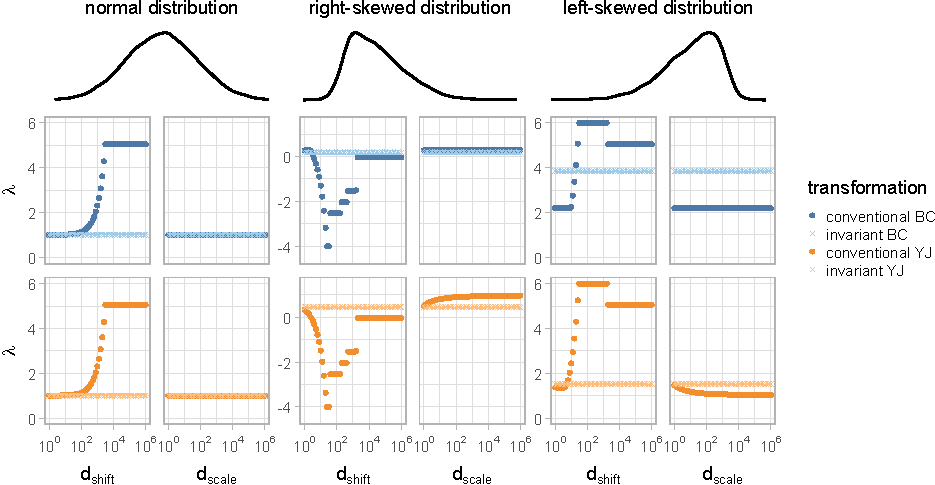
\includegraphics[width=1\linewidth]{figure_3} 

}

\caption{Invariant power transformation produces transformation parameters that are invariant to location and scale. Samples were drawn from normal, right-skewed and left-skewed distributions, respectively, which then underwent a shift $d_{\text{shift}}$ or multiplication by $d_{\text{scale}}$. Estimates of the transformation parameter $\lambda$ for the conventional power transformations show strong dependency on the overall location and scale of the distribution, whereas estimates obtained for the location- and scale-invariant power transformations are constant.}\label{fig:shifted-distributions}
\end{figure}

The result is shown in Figure \ref{fig:shifted-distributions}. For each
distribution, transformation parameter \(\lambda\) varied with
\(d_{\text{shift}}\) and \(d_{\text{scale}}\) when estimated for
conventional transformations. In contrast, estimation of \(\lambda\) for
invariant power transformations was invariant to both
\(d_{\text{shift}}\) and \(d_{\text{scale}}\).

\subsection{Robust transformations}\label{robust-transformations}

Outliers may be present in data and affect estimation of transformation
parameters. The log-likelihood function can be weighted to assign less
weight to outlier instances, see equations
\ref{eqn:box-cox-weighted-invariant-log-likelihood} and
\ref{eqn:yeo-johnson-weighted-invariant-log-likelihood}. We proposed
three weighting function: step, triangle and tapered cosine, that have
one, two and two parameters, respectively. Each weighting function then
takes one of three values as input: probabilities of the empirical
distribution of the original feature, the z-score of the transformed
feature values, or the residual error between the z-score of the
transformed feature values and their expected z-score based on the
normal distribution.

To determine the weighting function parameters for each of the nine
combinations, \(m_d=100\) asymmetric generalised normal distributions
were drawn. Each distribution was parametrised with a randomly chosen
skewness parameter \(\alpha \sim U\left(0.01, 0.99\right)\) and shape
parameter \(\beta \sim U\left(1.00, 5.00 \right)\). Location and scale
parameters were set as \(\mu = 0\) and \(\sigma = 1\), respectively.
\(n = \lceil 10^\gamma \rceil\) instances were then randomly drawn, with
\(\gamma \sim U\left(2, 4\right)\), i.e., between \(100\) and \(10000\)
values are drawn to create \(\mathbf{X}_i\).

Outlier values were then drawn to randomly replace a fraction of the
values of \(\mathbf{X}_i\). This was repeated \(m_{\text{out}} = 10\)
times, with outlier fractions regularly spaced in \([0.00, 0.10]\). Thus
up to 10 percent of the values could be replaced by outliers. Outlier
values were set according to \citet{Tukey1977-xm}, as follows. Let
\(x^{*} \sim U\left(-2, 2\right)\). Then the corresponding outlier value
was:

\begin{equation}
x_{out} =
\begin{cases}
Q_1 - \left(1.5 - x^{*} \right) \text{IQR} & \text{if } x^{*} < 0 \\
Q_3 + \left(1.5 + x^{*} \right) \text{IQR} & \text{if } x^{*} \geq 0
\end{cases}
\end{equation}

\(Q_1\), \(Q_3\) and \(\text{IQR}\) are the first quartile, third
quartile and interquartile range of \(\mathbf{X}_i\), respectively.
Outlier values randomly replaced values in \(\mathbf{X}_i\) to create
\(\mathbf{X}_{i,j}\), with
\(j \in \left\{ 1, \ldots, m_{\text{out}} \right\}\)

To find the optimal values for the weighting function parameters
\(\delta_1\) and \(\delta_2\) (if applicable), we minimised the absolute
difference between the \(\lambda_{r}\) parameter obtained for robust
transformation in the presence of outliers, and the \(\lambda_0\)
parameter obtained using the non-robust transformations in absence of
outliers:

\begin{equation}
\label{eqn:minimisation-weighting}
\left\{ \hat{\delta}_1, \hat{\delta}_2 \right\} = \argmin_{\delta_1, \delta_2} \sum_{i=1}^{m_d} \sum_{j=1}^{m_{\text{out}}} \left| \lambda_r \left(\mathbf{X}_{i, j}; \delta_1, \delta_2 \right) - \lambda_0 \left(\mathbf{X}_i \right) \right|
\end{equation}

Minimisation was conducted using the BOBYQA algorithm for
derivative-free bound constraint optimisation \citep{Powell2009-zb}. The
resulting weighting function parameters for weighted MLE are shown in
Tables \ref{tab:optimal-weighting-parameters-box-cox} and
\ref{tab:optimal-weighting-parameters-yeo-johnson} for robust location-
and scale-invariant Box-Cox and Yeo-Johnson transformations,
respectively.

\begin{table}
\begin{center}
\caption{Optimal weighting parameters and corresponding loss for location- and scale-invariant Box-Cox power transformations. $p^{*}$ indicates use of the empirical distribution of feature values, $z$ the z-score of the transformed feature values, and $r$ the residual error between the z-score of transformed feature values and the expected z-score according to the normal distribution. The \textit{initial} column shows the starting parameter value for the optimisation process, with the corresponding boundary values in the \textit{limits} column. The {optimal} column shows the optimal parameter values. The \textit{loss} column shows the loss achieved by each method, under optimised parameters. Lower loss indicates better robustness against outliers.}
\label{tab:optimal-weighting-parameters-box-cox}
\begin{tabular}{l r r r r r r r}

\toprule
method & \multicolumn{3}{c}{$\delta_1$} & \multicolumn{3}{c}{$\delta_2$} & loss \\
& initial & limits & optimal & initial & limits & optimal & \\

\midrule
non-robust               & ---  & ---       & ---  & ---  & ---       & ---  & 771 \\
$p^{*}$ (step)           & 0.80 & $(0, 1]$  & 0.86 & ---  & ---       & ---  & 561 \\
$p^{*}$ (triangle)       & 0.80 & $(0, 1]$  & 0.83 & 0.95 & $(0, 1]$  & 0.92 & 564 \\
$p^{*}$ (tapered cosine) & 0.80 & $(0, 1]$  & 0.76 & 0.95 & $(0, 1]$  & 0.95 & 560 \\
$z$ (step)               & 1.28 & $(0, 10]$ & 1.12 & ---  & ---       & ---  & 1153 \\
$z$ (triangle)           & 1.28 & $(0, 10]$ & 0.38 & 1.96 & $(0, 10]$ & 4.48 & 1178 \\
$z$ (tapered cosine)     & 1.28 & $(0, 10]$ & 1.21 & 1.96 & $(0, 10]$ & 4.92 & 1135 \\
$r$ (step)               & 0.50 & $(0, 10]$ & 2.18 & ---  & ---       & ---  & 1839 \\
$r$ (triangle)           & 0.50 & $(0, 10]$ & 1.29 & 1.00 & $(0, 10]$ & 1.47 & 1764 \\
$r$ (tapered cosine)     & 0.50 & $(0, 10]$ & 1.38 & 1.00 & $(0, 10]$ & 1.41 & 1583 \\
\bottomrule
\end{tabular}
\end{center}
\end{table}

\begin{table}
\begin{center}
\caption{Optimal weighting parameters and corresponding loss for location- and scale-invariant Yeo-Johnson power transformations. $p^{*}$ indicates use of the empirical distribution of feature values, $z$ the z-score of the transformed feature values, and $r$ the residual error between the z-score of transformed feature values and the expected z-score according to the normal distribution. The \textit{initial} column shows the starting parameter value for the optimisation process, with the corresponding boundary values in the \textit{limits} column. The {optimal} column shows the optimal parameter values. The \textit{loss} column shows the loss achieved by each method, under optimised parameters. Lower loss indicates better robustness against outliers.}
\label{tab:optimal-weighting-parameters-yeo-johnson}
\begin{tabular}{l r r r r r r r}

\toprule
method & \multicolumn{3}{c}{$\delta_1$} & \multicolumn{3}{c}{$\delta_2$} & loss \\
& initial & limits & optimal & initial & limits & optimal & \\

\midrule
non-robust               & ---  & ---       & ---  & ---  & ---       & ---  & 364 \\
$p^{*}$ (step)           & 0.80 & $(0, 1]$  & 0.95 & ---  & ---       & ---  & 224 \\
$p^{*}$ (triangle)       & 0.80 & $(0, 1]$  & 0.88 & 0.95 & $(0, 1]$  & 0.97 & 212 \\
$p^{*}$ (tapered cosine) & 0.80 & $(0, 1]$  & 0.94 & 0.95 & $(0, 1]$  & 0.95 & 218 \\
$z$ (step)               & 1.28 & $(0, 10]$ & 1.09 & ---  & ---       & ---  & 392 \\
$z$ (triangle)           & 1.28 & $(0, 10]$ & 0.24 & 1.96 & $(0, 10]$ & 4.62 & 396 \\
$z$ (tapered cosine)     & 1.28 & $(0, 10]$ & 0.15 & 1.96 & $(0, 10]$ & 6.05 & 413 \\
$r$ (step)               & 0.50 & $(0, 10]$ & 1.63 & ---  & ---       & ---  & 746 \\
$r$ (triangle)           & 0.50 & $(0, 10]$ & 1.50 & 1.00 & $(0, 10]$ & 1.79 & 731 \\
$r$ (tapered cosine)     & 0.50 & $(0, 10]$ & 1.51 & 1.00 & $(0, 10]$ & 1.57 & 612 \\
\bottomrule
\end{tabular}
\end{center}
\end{table}

Figure \ref{fig:optimised-weighting-function-parameters} shows the
distribution of errors \(\left| \lambda_r - \lambda_0 \right|\) for
non-robust and robust transformations using the optimal weighting
function parameters. In the presence of outliers, the Yeo-Johnson
transformation yielded smaller errors than the Box-Cox transformation.
For both transformations, weighting based on empirical probabilities
yielded the most consistent \(\lambda\) parameter estimates in the
presence of outliers. Other methods did not outperform the non-robust
transformation method.

\begin{figure}

{\centering 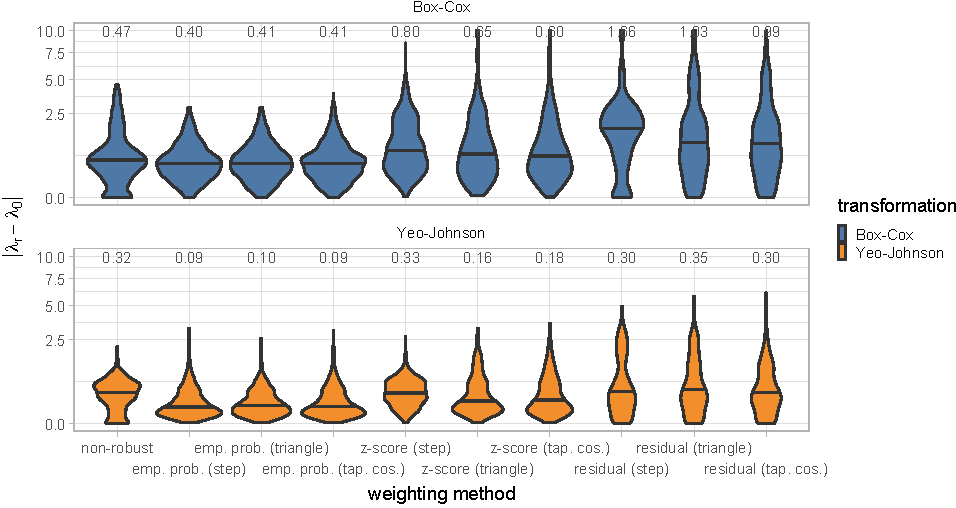
\includegraphics[width=1\linewidth]{figure_4} 

}

\caption{Robustness of power transformations after optimising weighting function parameters. The distribution of errors, i.e. the difference between robustly fitted $\lambda^r$ and expected $\lambda_{0}$ found in the absence of outliers, is shown for 1000 randomly parametrised asymmetric generalised normal distributions with up to 10\% outliers on either side of the distribution. The top and bottom panel show errors for the location- and scale-invariant Box-Cox and Yeo-Johnson transformations, respectively. In each panel, the error distribution for the non-robust transformation is shown to the left for comparison with different weighting methods. Note that a square root transformation was applied along the $y$-axis for display purposes. Median errors are shown above each distribution.}\label{fig:optimised-weighting-function-parameters}
\end{figure}

\subsection{Empirical central normality
test}\label{empirical-central-normality-test-1}

To develop an empirical test for central normality we need to consider
two parameters: the central portion \(\kappa\) as a fixed parameter, and
test statistic \(\tau_{\text{ecn}}\). We will first define the central
portion \(\kappa\).

First we draw \(m_d=10000\) random asymmetric generalised normal
distributions. As before, each distribution is parametrised with a
randomly chosen skewness parameter
\(\alpha \sim U\left(0.01, 0.99\right)\) and shape parameter
\(\beta \sim U\left(1.00, 5.00 \right)\). Location and scale parameters
are set as \(\mu = 0\) and \(\sigma = 1\), respectively.
\(n = \lceil 10^\gamma \rceil\) values are then randomly drawn, with
\(\gamma \sim U\left(1.47, 3.00\right)\), which leads to between \(30\)
and \(1000\) values being drawn to create \(\mathbf{X}_i\). As before,
for each distribution, up to \(10 \%\) of instances are replaced by
outlier values, and this is repeated \(10\) times. We then compute
residuals after optimising robust location- and scale-invariant
transformations with the empirical tapered cosine weighting method.

Figure \ref{fig:empirical-central-normality-residual-error} shows the
residual errors of the transformed distribution as function of the
empirical probability. As expected, the largest deviations from
normality appear on the extremities of this range. For Box-Cox
transformations, the effect of outliers on the lower end of the
distribution leads to noticeable asymmetry. Between very low and very
high empirical probabilities, residual errors are constrained and
relatively flat. This is the candidate range for the central portion of
the data.

\begin{figure}

{\centering 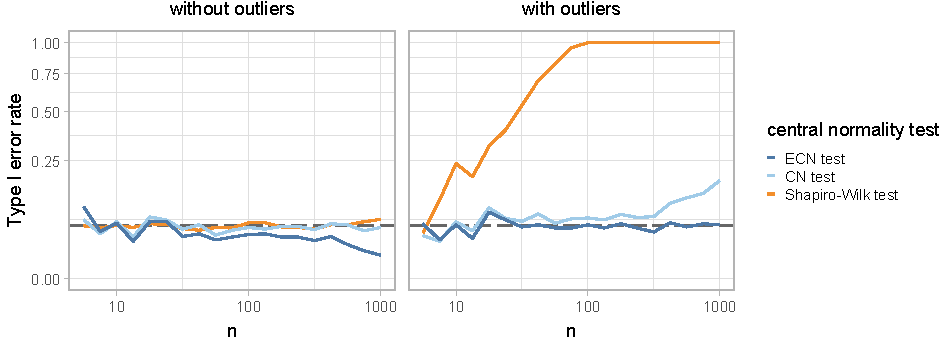
\includegraphics[width=1\linewidth]{figure_5} 

}

\caption{Residual error as a function of empirical probability. Percentiles of the error are shown for robust, location- and scale-invariant transformations of 10000 randomly drawn asymmetric generalised normal distributions, for each of which outliers were randomly drawn 10 times (up to 10\% of samples). Larger errors occur at the edges of each distribution.}\label{fig:empirical-central-normality-residual-error}
\end{figure}

We then consider the empirical probability of type I errors: the
probability of incorrectly classifying a centrally normal distribution
as being non-normal based on the test statistic \(\tau_{\text{ecn}}\).
Under the assumption that the asymmetric generalised normal
distributions are centrally normal after robust transformation, this
produces the relationship shown in Figure
\ref{fig:empirical-central-normality-type-1-error-rate}. Since for
\(\kappa \leq 0.80\) error curves for both transformation methods are
similar, we fix the value of the central portion \(\kappa\) to 0.80. In
the remaining we will use the empirical central normality test statistic
values defined using robust location- and scale-invariant Yeo-Johnson
transformations, as it is more conservative (see \ref{appendix-e-empirical-central-normality-test}). This leads
to test statistic values listed in Table
\ref{tab:empirical-central-normality}

\begin{figure}

{\centering 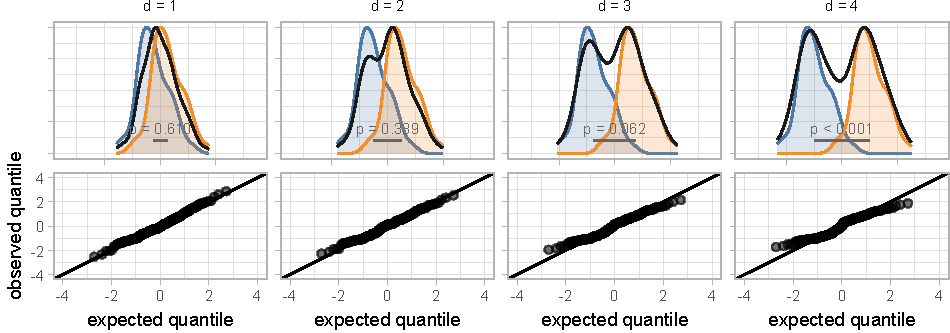
\includegraphics[width=1\linewidth]{figure_6} 

}

\caption{Type 1 error rate of transformed asymmetric generalised normal distributions as function of the test statistic $\tau_{\text{ecn}}$ for the central portion $\kappa$ of the distribution.}\label{fig:empirical-central-normality-type-1-error-rate}
\end{figure}

\begin{table}
\begin{center}
\caption{Test statistic $\tau_{\text{ecn}}$ for empirical central normality at $\kappa = 0.80$ as a function of Type I error rate.}
\label{tab:empirical-central-normality}
\begin{tabular}{l | c c c c c c c}

\toprule
type I error rate & 0.50 & 0.20 & 0.10 & 0.05 & 0.02 & 0.01 & 0.001 \\

\midrule
$\tau_{\text{ecn}}$ & 0.041 & 0.062 & 0.075 & 0.088 & 0.103 & 0.115 & 0.154 \\
\bottomrule
\end{tabular}
\end{center}
\end{table}

In Figure \ref{fig:empirical-central-normality-examples} we apply the
empirical central normality test to assess central normality of features
that are composed of a mixture of samples drawn from two normal
distributions. With increased separation of the underlying normal
distributions, the probability of the feature being centrally normal
decreases, as expected.

\begin{figure}

{\centering 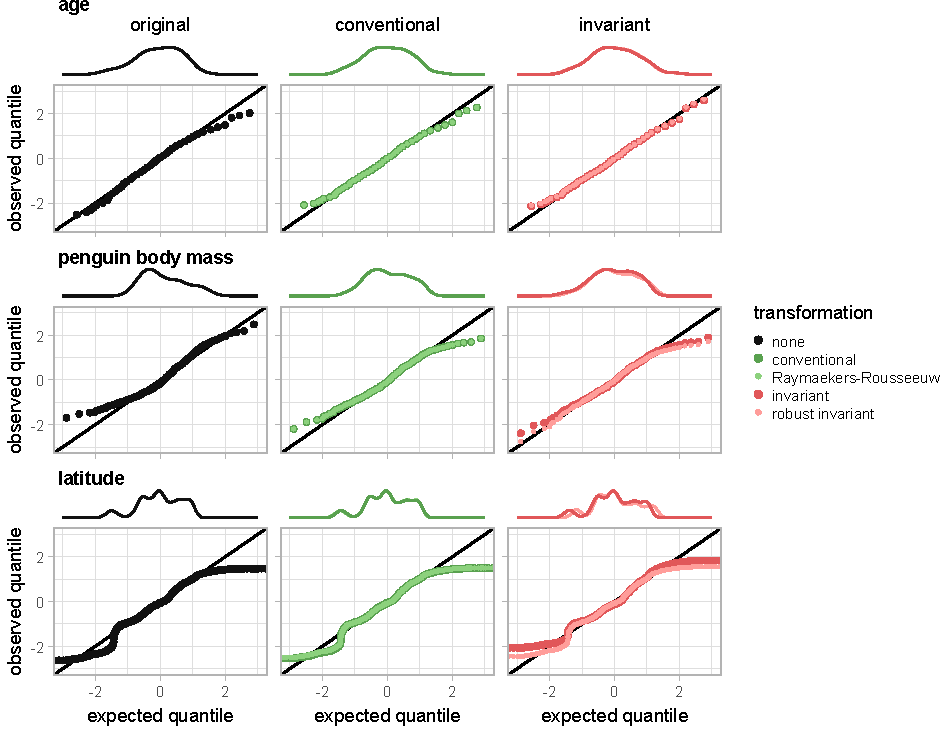
\includegraphics[width=1\linewidth]{figure_7} 

}

\caption{Bi-modal distributions and empirical central normality test results. The feature (black) is a mixture of two identical sample sets (blue and orange) drawn from normal distributions that are offset by a distance $d$. We use the empirical centrally normality test to compute the probability for the hypothesis that the distribution is centrally normal. As may be observed, with increasing offset $d$ the probability that the feature is centrally normal decreases. Quantile-quantile plots are drawn below each distribution.}\label{fig:empirical-central-normality-examples}
\end{figure}

\section{Experimental Results}\label{experimental-results}

\subsection{Invariance}\label{sec:invariance}

Location- and scale-invariant power transformations are intended to
yield improved transformations to normality in the presence of large
shifts in location, distributions that due to location and scale are not
centered near zero, or both. Earlier, we assessed these transformations
using simulated data. In the following, they are evaluated using
examples from real datasets. We focus on the Yeo-Johnson transformation
because of its ability to handle features with negative values. Results
for Box-Cox transformations are shown in 
\ref{appendix-d-experimental-results-using-location--and-scale-invariant-box-cox-transformation}.

\begin{figure}

{\centering 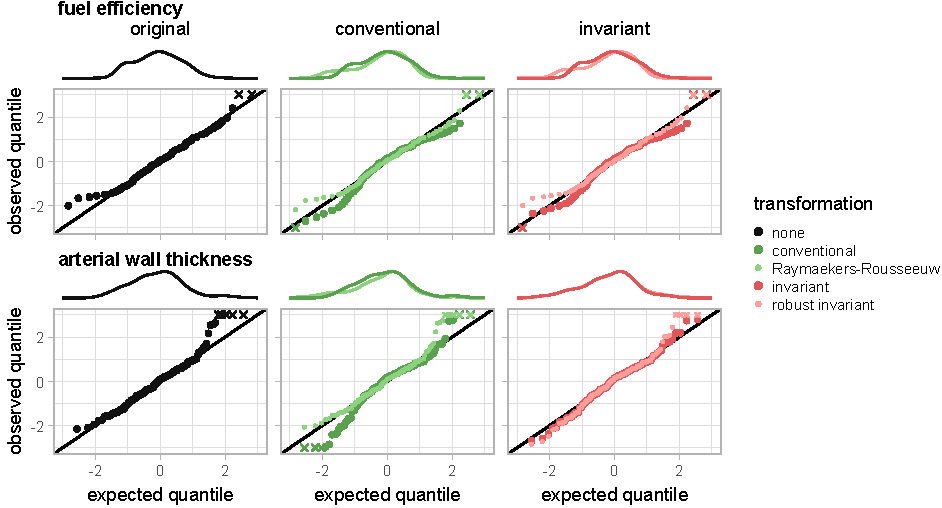
\includegraphics[width=1\linewidth]{figure_8} 

}

\caption{Quantile-quantile plots for several datasets: age of patients with lung cancer (top row); penguin body mass (middle row); and latitude coordinates of houses sold in Ames, Iowa (bottom row). Multiple quantile-quantile plots are shown: for the original feature (left column); the feature transformed using the conventional Yeo-Johnson transformation and Raymaekers and Rousseeuw's robust adaptation (middle column); and the feature transformed using the non-robust and robust location- and-scale invariant Yeo-Johnson transformations (right column).}\label{fig:experimental-results-invariance}
\end{figure}

\subsubsection{Age of patients with lung
cancer}\label{sec:age-of-patients-with-lung-cancer}

A common feature in health-related datasets is age. Here we use data on
228 patients with lung cancer that was collected and published by
Loprinzi et al. \citep{Loprinzi1994-cd}. The age in the cohort was
\(62.4 \pm 9.1\) (mean ± standard deviation) years. Applying
conventional and invariant Yeo-Johnson transformations to patient age
yielded the following results, see Figure
\ref{fig:experimental-results-invariance}: no transformation (sum of
residuals with normal distribution \(\sum r_i = 16.5\)); conventional
transformation (\(\lambda = 2.0\), \(\sum r_i = 11.5\),
\(\mu_{YJ} = 1.8 \cdot 10^3\), \(\sigma_{YJ} = 0.5 \cdot 10^3\));
Raymaekers and Rousseeuw's robust adaptation (\(\lambda = 2.0\),
\(\sum r_i = 11.5\), \(\mu_{YJ} = 1.8 \cdot 10^3\),
\(\sigma_{YJ} = 0.5 \cdot 10^3\)); location- and scale-invariant
transformation (\(\lambda = 0.9\), \(\sum r_i = 8.8\),
\(\mu_{YJ} = 1.2\), \(\sigma_{YJ} = 1.1\)); and robust location- and
scale-invariant transformation (\(\lambda = 0.8\), \(\sum r_i = 10.6\),
\(\mu_{YJ} = 1.2\), \(\sigma_{YJ} = 1.0\)).

Location- and scale-invariant transformation led to a lower overall
residual sum, indicating a better transformation. Robust location- and
scale-invariant transformation had a higher residual sum compared to the
non-robust variant, which may be due to the lack of outliers in the
data. Conventional transformations inflated the mean \(\mu_{YJ}\) and
standard deviation \(\sigma_{YJ}\) of the age feature after
transformation. The empirical central normality test did not detect any
statistically significant deviations from central normality for any
transformation (all \(p \geq 0.78\)).

\subsubsection{Penguin body mass}\label{sec:penguin-body-mass}

Gorman, Williams and Fraser recorded body mass (in grams) of 342
penguins of three different species \citep{Gorman2014-eo}.
The body mass was \((4.2 \pm 0.8) \cdot 10^3\) (mean ± standard
deviation) grams, and not centrally normal (\(p = 0.03\)). Applying
conventional and invariant Yeo-Johnson transformations to body mass
yielded the following results, see Figure
\ref{fig:experimental-results-invariance}: no transformation (residual
sum \(\sum r_i = 48.0\)); conventional transformation
(\(\lambda = -0.5\), \(\sum r_i = 32.2\), \(\mu_{YJ} = 2.1\),
\(\sigma_{YJ} = 4 \cdot 10^{-3}\)); Raymaekers and Rousseeuw's robust
adaptation (\(\lambda = -0.5\), \(\sum r_i = 32.2\), \(\mu_{YJ} = 2.1\),
\(\sigma_{YJ} = 4 \cdot 10^{-3}\)); location- and scale-invariant
transformation (\(\lambda = 0.5\), \(\sum r_i = 26.8\),
\(\mu_{YJ} = 0.9\), \(\sigma_{YJ} = 0.9\)); and robust location- and
scale-invariant transformation (\(\lambda = 0.4\), \(\sum r_i = 23.1\),
\(\mu_{YJ} = 0.8\), \(\sigma_{YJ} = 0.8\)).

Location- and scale-invariant transformation produced a lower overall
residual sum, indicating a better transformation. Moreover, conventional
transformations led to low standard deviation \(\sigma_{YJ}\) of the
body mass feature after transformation. The empirical central normality
test did not detect any statistically significant deviations from
central normality for any transformation (all \(p \geq 0.38\)).

\subsubsection{Latitude in the Ames housing
dataset}\label{sec:latitude-in-the-ames-housing-dataset}

Geospatial datasets usually contain coordinates. The Ames housing
dataset contains data on 2930 properties that were sold between 2006 and
2010 \citep{De-Cock2011-jf} including their geospatial coordinates. The
latitude was \(42.03 \pm 0.02)\) (mean ± standard deviation). Applying
conventional and invariant Yeo-Johnson transformations to latitude
yielded the following results, see Figure
\ref{fig:experimental-results-invariance}: no transformation (residual
sum \(\sum r_i = 328\)); conventional transformation
(\(\lambda = 62.1\), \(\sum r_i = 319\),
\(\mu_{YJ} = 4.8 \cdot 10^{99}\), \(\sigma_{YJ} = 0.1 \cdot 10^{99}\));
Raymaekers and Rousseeuw's robust adaptation (\(\lambda = 95.4\),
\(\sum r_i = 319\), \(\mu_{YJ} = 6.4 \cdot 10^{153}\),
\(\sigma_{YJ} = 0.3 \cdot 10^{153}\)); location- and scale-invariant
transformation (\(\lambda = 1.5\), \(\sum r_i = 326\),
\(\mu_{YJ} = -1.2\), \(\sigma_{YJ} = 0.8\)); and robust location- and
scale-invariant transformation (\(\lambda = 1.4\), \(\sum r_i = 311\),
\(\mu_{YJ} = -1.3\), \(\sigma_{YJ} = 0.9\)).

Every transformation reduced the residual sum. The non-robust location-
and scale-invariant transformation did not improve over conventional
alternatives and yielded a data distribution lacking central normality
(empirical central normality test: \(p=0.05\)). However, conventional
transformations had high values for the \(\lambda\) parameter, which
could lead to numerical issues.

\subsection{Robustness against
outliers}\label{sec:robustness-against-outliers}

We previously simulated data to assess invariant power transformations
and their robustness against outliers. Here, we assess invariant power
transformations in real data with outliers.

\begin{figure}

{\centering 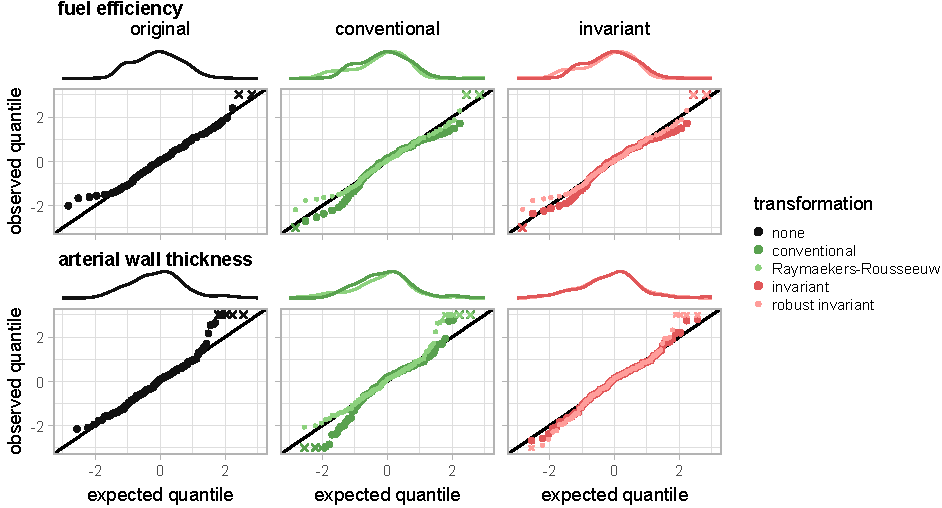
\includegraphics[width=1\linewidth]{figure_9} 

}

\caption{Quantile-quantile plots for two datasets with outliers: vehicle fuel consumption (top row), where outliers are related to highly fuel-efficient vehicles; and maximum arterial wall thickness in patients with ischemic stroke (bottom row). Multiple quantile-quantile plots are shown: for the original feature (left column); the feature transformed using the conventional Yeo-Johnson transformation and Raymaekers and Rousseeuw's robust adaptation (middle column); and the feature transformed using the non-robust and robust location- and-scale invariant Yeo-Johnson transformations (right column). Samples with observed quantiles below $-3.0$ or above $3.0$ are indicated by crosses.}\label{fig:experimental-results-outlier-robustness}
\end{figure}

\subsubsection{Fuel efficiency in the Top Gear
dataset}\label{sec:fuel-efficiency-in-the-top-gear-dataset}

The Top Gear dataset contains data on 297 vehicles that appeared on the
BBC television show \emph{Top Gear} \citep{Alfons2021-kc}. Within this dataset,
the fuel consumption feature contains outliers due to highly
fuel-efficient vehicles. Applying conventional and invariant Yeo-Johnson
transformations to the fuel consumption feature yielded the following
results, see Figure \ref{fig:experimental-results-outlier-robustness}:
no transformation (residual sum \(\sum r_i = 54\), \(p=0.76\));
conventional transformation (\(\lambda = -0.1\), \(\sum r_i = 55\),
\(\mu_{YJ} = 3.0\), \(\sigma_{YJ} = 0.3\), \(p=0.01\)); Raymaekers and
Rousseeuw's robust adaptation (\(\lambda = 0.8\), \(\sum r_i = 48\),
\(\mu_{YJ} = 29\), \(\sigma_{YJ} = 15\), \(p=0.55\)); location- and
scale-invariant transformation (\(\lambda = -1.3\), \(\sum r_i = 44\),
\(\mu_{YJ} = 0.5\), \(\sigma_{YJ} = 0.1\), \(p=0.03\)); and robust
location- and scale-invariant transformation (\(\lambda = -0.9\),
\(\sum r_i = 50\), \(\mu_{YJ} = 2.0\), \(\sigma_{YJ} = 2.3\),
\(p=0.58\)).

Outliers cause non-robust transformations to fail to transform the data
to a centrally normal distribution (empirical central normality test
\(p = 0.01\) and \(p=0.03\) for conventional and invariant
transformations, respectively). Robust transformations produce
distributions that are centrally normal (empirical central normality
test \(p > 0.05\)).

\subsubsection{Maximum arterial wall thickness in an ischemic stroke
dataset}\label{sec:maximum-arterial-wall-thickness-in-an-ischemic-stroke-dataset}

The ischemic stroke dataset contains historic data from 126 patients
with risk at ischemic stroke \citep{Kuhn2019-kt}. These patients
underwent Computed Tomography Angiography to characterize the carotid
artery blockages. Angiography imaging was then assessed, and various
characteristics related to the blood vessels and the disease are
measured. The maximum arterial wall thickness feature contains several
instances with outlier values. Applying conventional and invariant
Yeo-Johnson transformations to this feature yielded the following
results, see Figure \ref{fig:experimental-results-outlier-robustness}:
no transformation (residual sum \(\sum r_i = 110\), \(p=0.56\));
conventional transformation (\(\lambda = -0.7\), \(\sum r_i = 30\),
\(\mu_{YJ} = 1.0\), \(\sigma_{YJ} = 0.1\), \(p=0.01\)); Raymaekers and
Rousseeuw's robust adaptation (\(\lambda = 1.1\), \(\sum r_i = 136\),
\(\mu_{YJ} = 7.2\), \(\sigma_{YJ} = 14\), \(p=0.61\)); location- and
scale-invariant transformation (\(\lambda = 0.2\), \(\sum r_i = 12\),
\(\mu_{YJ} = -11.8\), \(\sigma_{YJ} = 6.9\), \(p=0.13\)); and robust
location- and scale-invariant transformation (\(\lambda = -0.6\),
\(\sum r_i = 27\), \(\mu_{YJ} = 0.7\), \(\sigma_{YJ} = 0.1\),
\(p=0.10\)).

Non-robust transformations failed to produce a centrally normal
distribution (empirical central normality test \(p=0.01\) and \(p=0.02\)
for conventional and invariant transformations, respectively). Robust
transformations produce distributions that are centrally normal
(empirical central normality test \(p > 0.05\)).

\subsection{Integration into end-to-end machine
learning}\label{integration-into-end-to-end-machine-learning}

We used 285 datasets from the Penn Machine Learning Benchmarks
collection \citep{Romano2022-gq}. In this collection, 122 datasets
correspond to regression tasks and 163 datasets to classification tasks.
Using the familiar auto-machine learning library (version 1.5.0) \citep{Zwanenburg2021-so},
each dataset was used to train a model for each
of 16 process configurations. Each process configuration specifies the
learner (generalised linear model or random forest), transformation
method (none, conventional Yeo-Johnson, robust invariant Yeo-Johnson,
robust invariant Yeo-Johnson with empirical central normality test
(rejecting transformations with \(p \leq 0.01\)), and normalisation
method (none, \(z\)-standardisation), yielding 16 distinct
configurations. Before each experiment, each dataset was randomly split
into a training (70\%) and holdout test (30\%) set five times. Thus, a
total of 22800 models were created. Each model was then evaluated using
the holdout test set using one of two metrics, i.e.~the root relative
squared error (RRSE) for regression tasks and the area under the
receiver operating characteristic curve (AUC) for classification tasks.

For the purpose of assessing the effect of the difficulty of the task,
we computed the median performance score over all models for each
dataset and assigned one the following categories:

\begin{itemize}
\item
  very easy: \(\text{AUC} \geq 0.90\) or \(\text{RRSE} \leq 0.10\) (87
  datasets)
\item
  easy: \(0.90 > \text{AUC} \geq 0.80\) or
  \(0.30 \geq \text{RRSE} > 0.10\) (46 datasets)
\item
  intermediate: \(0.80 > \text{AUC} \geq 0.70\) or
  \(0.60 \geq \text{RRSE} > 0.30\) (72 datasets)
\item
  difficult: \(0.70 > \text{AUC} \geq 0.60\) or
  \(0.80 \geq \text{RRSE} > 0.60\) (60 datasets)
\item
  very difficult: \(0.60 > \text{AUC} \geq 0.50\) or
  \(1.00 \geq \text{RRSE} > 0.80\) (12 datasets)
\item
  unsolvable: \(\text{AUC} < 0.50\) or \(\text{RRSE} > 1.00\) (8
  datasets)
\end{itemize}

To remove the effect of the dataset, and allow for comparing metrics, we
ranked all performance scores for each dataset so that a higher rank
corresponds to better performance. Experiments yielding the same score
received the same, average, rank. Subsequently ranks were normalised to
the \([0.0, 1.0]\) range.

Significant differences exist between process configurations (Friedman
test: \(p < 10^{-8})\).

Here we focus on the subset of 232 datasets that contain numeric
features. Considering single process parameters, the choice of learner
(Wilcoxon signed rank test: \(p < 10^{-8})\)) and normalisation method
(Wilcoxon signed rank test: \(p = 0.007\)) had a significant impact (at
significance level \(p = 0.050\)), but transformation method (Friedman
test: \(p = 0.054\)) did not.

To estimate the marginal effects of process parameters, including
transformation method, we first fit a regression random forest (ranger
package version 0.16.0, \citep{Wright2017-rf}): 2000 trees, minimum
node size 2, other hyperparameters default) with process parameters and
task difficulty as predictors and normalised rank as response variable.
The estimated marginal effects are shown in Figure
\ref{fig:marginal-effect-plot}. On the scale of normalised ranks
(\([0.0, 1.0]\)), the overall estimated marginal effect of using a
random forest instead of generalised linear model was \(0.272\). The
overall marginal effect of using z-standardisation to normalise features
was \(0.008\). Transformation methods had the following marginal
effects: \(0.003\) for using conventional Yeo-Johnson transformation
instead of no transformation; \(-0.007\) for using robust invariant
Yeo-Johnson transformation instead of no transformation; \(-0.009\) for
using robust invariant Yeo-Johnson transformation with empirical central
normality test instead of no transformation; \(-0.010\) for using robust
invariant Yeo-Johnson transformation instead of conventional Yeo-Johnson
transformation; and \(-0.012\) for using using robust invariant
Yeo-Johnson transformation with empirical central normality test instead
of conventional Yeo-Johnson transformation.

\begin{figure}

{\centering 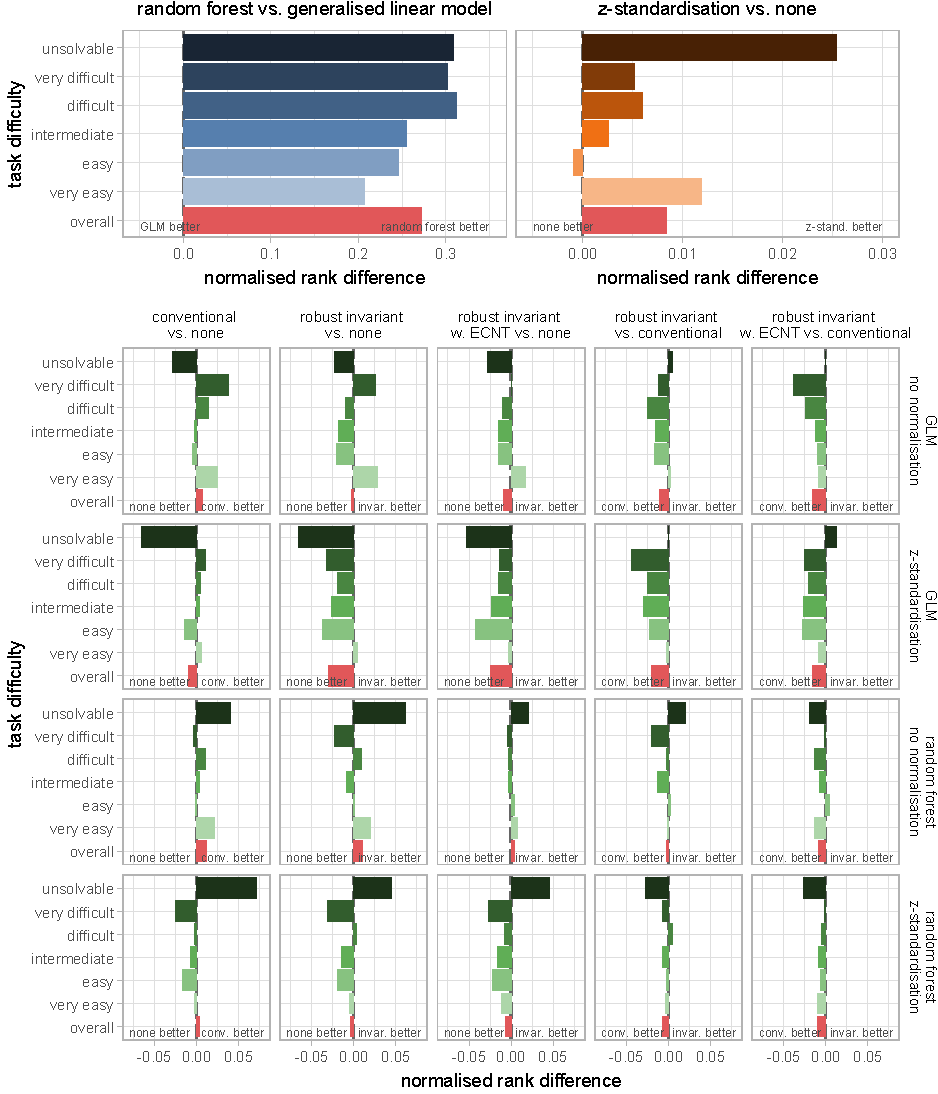
\includegraphics[width=1\linewidth]{figure_10} 

}

\caption{Estimated marginal effect of learners, normalisation and transformation methods on ranked model performance scores in 18560 machine learning experiments on 232 datasets. The top-left panel shows the marginal effect of learners, i.e. random forests and generalised linear models (GLM). Random forests outperform GLM models for all task difficulties. The top-right panel shows the marginal effect of feature normalisation methods, i.e. no normalisation and z-standardisation. z-standardisation is generally beneficial, but the estimated effect is neglible. The bottom panel shows the marginal effects of different transformation methods, split by learner and normalisation method. There is no consistent behaviour, and estimated effects are neglible. Note that the ranges of the $x$-axes of the three main panels differ. ECNT: empirical central normality test.}\label{fig:marginal-effect-plot}
\end{figure}

\section{Discussion}\label{discussion}

In their work on power transformation, Box and Cox already mention
transformation with a shift parameter, but preferred the version in Eq.
\ref{eqn:box-cox-original} for the theoretical analysis in their paper
\citep{Box1964-mz}, which subsequently became the convention. Yeo and
Johnson's power transformation lacks a shift parameter altogether 
\citep{Yeo2000-vw}. We showed that these power transformations are
sensitive to location and scale of data distributions. To mitigate this
issue, we defined location- and scale-invariant variants of the Box-Cox
and Yeo-Johnson transformations. We furthermore assessed methods for
making these transformations robust to outliers, and devised an
empirical test for central normality.

Robust location- and scale-invariant transformations are a suitable
replacement for their conventional counterparts. They demonstrated
robustness against outliers and prevent inaccurate transformations and
potential numerical issues due to location and scale of the distribution
of a feature. This is particularly relevant for automated data
processing, where such issues may go unnoticed. Compared to non-robust
location- and scale-invariant transformations, real-world examples with
outliers showed higher residual errors of transformed features. Robust
transformations seek to minimise residual errors for the central part of
the distribution, instead of the entire distribution, including
outliers. The empirical central normality test indicated that robust
transformations are better able to achieve central normality in the
presence of outliers. However, in a machine learning experiment of 232
real-world datasets that contained at least one numeric feature, we did
not find a meaningful benefit -- nor detriment -- to model performance
for location- and scale-invariant power transformations. One reason may
be that numeric features with large location shifts (\(|\mu| > 1000.0\))
were uncommon. Of the 4886 numeric features in the 232 datasets, 266
(5\%) features in 34 datasets had large location shifts, of which 200
appeared in just 2 datasets. For the latter two datasets, the
transformation method did not show significant difference between groups
(Friedman test; \(p > 0.05\)).

Location- and scale-invariant transformations are realised by
simultaneously optimising three parameters, i.e.~transformation
parameter \(\lambda\), shift parameter \(x_0\) and scale parameter
\(s\). We derived the log-likelihood function to facilitate optimisation
using MLE. Alternatively, standardisation of a numeric variable (e.g.,
through subtracting its median value and division by its interquartile
range) prior to conventional power transformations may achieve a similar
effect in reducing sensitivity to the distribution's location and scale.
While this alternative helps prevent these issues -- provided that
normalisation does not lead to negative values for Box-Cox
transformation -- location- and scale-invariant transformations seem to
provide an overall better transformation to normality 
(\ref{appendix-f-normalisation-before-transformation}).

We assessed several methods for robust power transformation. Methods
that relied on the z-score of the transformed feature or the residual
error yielded worse results than the non-robust method. This is partly
due to the initial choice of threshold parameters. Using different
initial values, closer to the upper limits
(\(\delta_1 = 10.0; \delta_2 = 10.0\)), led to a reduced loss. However,
these values effectively correspond to a non-robust transformation,
where all instances receive the same weight. Underperformance of these
methods could be explained by their use of transformed features for
setting weights. Consequently, the weights change at each iteration in
the MLE optimisation process. This increases local variance in the
log-likelihood function and creates local optima that the optimiser may
not handle well. As a consequence, optimal values for transformation
parameter \(\lambda\) might differ, which increases the presented loss
for optimising threshold parameters. Methods that relied on the
empirical probability did not suffer from this issue, as weights
remained fixed during MLE.

We introduced an empirical test for central normality to assess whether
distributions deviate from normality in a way that might require closer
inspection prior to further processing. The empirical test for central
normality differs from other tests for normality, such as the
Shapiro-Wilk test \citep{Shapiro1965-zd}, in that the test statistic is
independent of the number of samples. This makes this test more
practical for assessing central normality for larger sample numbers,
where other tests may detect inconsequential deviations from normality.

This work has the following limitations. Firstly, we did observe several
numerical stability issues for optimisation criteria other than MLE
(\ref{appendix-b-optimisation-of-transformation-parameters}).
These appear in regions where transformation parameters
would lead to very large or small numbers when using conventional power
transformations. For MLE stability issues were not observed. Secondly,
the empirical central normality test is based on simulations instead of
statistical theory, and relies on a somewhat arbitrary definition of the
central portion of a distribution. Thus, while the test may asses
whether data is sufficiently normally distributed for practical
purposes, it should not be used as a strict test for normality.

\section{Conclusion}\label{conclusion}

Compared to their conventional versions, robust location- and
scale-invariant Box-Cox and Yeo-Johnson transformations reduce
sensitivity to outliers and the location and scale of features. An
empirical central normality test can assess the quality of
transformation of features to normal distributions. The combination of
both facilitate the use of power transformations in automated data
analysis workflows.

\section{Data and code availability}\label{data-and-code-availability}

Location- and scale-invariant power transformations were implemented in
the \texttt{power.transform} package for R, which is available from
GitHub (https://github.com/oncoray/power.transform) and the CRAN
repository (https://cran.r-project.org/package=power.transform).
The manuscript was created using R Markdown and is likewise
available from the \texttt{power.transform} GitHub repository. Data and
results for the machine learning experiment are separately available
from Zenodo (https://doi.org/10.5281/zenodo.13736671).

\section{Acknowledgements}\label{sec:acknowledgments}

This research did not receive any specific grant from funding agencies in the public, commercial, or not-for-profit sectors.

%% The Appendices part is started with the command \appendix;
%% appendix sections are then done as normal sections
\appendix
\section{Log-likelihood functions for location and scale
invariant power transformation}\label{appendix-a-log-likelihood-functions-for-location-and-scale-invariant-power-transformation}

Location and scale-invariant Box-Cox and Yeo-Johnson transformations are
parametrised using location \(x_0\) and scale \(s\) parameters, in
addition to transformation parameter \(\lambda\). This leads to the
following transformations. The location and scale-invariant Box-Cox
transformation is:

\begin{equation}
\phi_{\text{BC}}^{\lambda, x_0, s} (x_i) = 
\begin{cases}
\left( \left(\frac{x_i - x_0}{s} \right)^\lambda - 1 \right) / \lambda & \text{if } \lambda \neq 0\\
\log\left[\frac{x_i - x_0}{s}\right] & \text{if } \lambda = 0
\end{cases}
\end{equation}

where \(x_i - x_0 > 0\). The location and scale-invariant Yeo-Johnson
transformation is:

\begin{equation}
\phi_{\text{YJ}}^{\lambda, x_0, s} (x_i) = 
\begin{cases}
\left( \left( 1 + \frac{x_i - x_0}{s}\right)^\lambda - 1\right) / \lambda & \text{if } \lambda \neq 0 \text{ and } x_i - x_0 \geq 0\\
\log\left[1 + \frac{x_i - x_0}{s}\right] & \text{if } \lambda = 0 \text{ and } x_i - x_0 \geq 0\\
-\left( \left( 1 - \frac{x_i - x_0}{s}\right)^{2 - \lambda} - 1 \right) / \left(2 - \lambda \right) & \text{if } \lambda \neq 2 \text{ and } x_i - x_0 < 0\\
-\log\left[1 - \frac{x_i - x_0}{s}\right] & \text{if } \lambda = 2 \text{ and } x_i - x_0 < 0
\end{cases}
\end{equation}

The parameters of these power transformations can be optimised based by
maximising the log-likelihood function, under the assumption that the
transformed feature \(\phi^{\lambda, x_0, s} (\mathbf{X})\) follows a
normal distribution. The log-likelihood functions for conventional
Box-Cox and Yeo-Johnson transformations are well-known. However, the
introduction of scaling parameter \(s\) prevents their direct use. Here,
we first derive the general form of the log-likelihood functions, and
then derive their power-transformation specific definitions.

Let \(f(x_1, \ldots, x_n)\) be the probability density function of
feature \(\mathbf{X} = \{ x_1, \ldots, x_n\}\), and
\(f^{\lambda, x_0, s} (\phi^{\lambda, x_0, s}(x_1), \ldots, \phi^{\lambda, x_0, s}(x_n))\)
be the probability density function of the transformed feature
\(\phi^{\lambda, x_0, s} (\mathbf{X})\), that is assumed to follow a
normal distribution.

The two probability density functions are related as follows:

\begin{equation}
f^{\lambda, x_0, s}(x_1, \ldots, x_n) = f^{\lambda, x_0, s} (\phi^{\lambda, x_0, s}(x_1), \ldots, \phi^{\lambda, x_0, s}(x_n)) \left|\mathbf{J}\right|
\end{equation}

Where, \(\left|\mathbf{J}\right|\) is the determinant of Jacobian
\(\mathbf{J}\). The Jacobian takes the following form, with off-diagonal
elements \(0\):

\begin{equation}
\mathbf{J} =
\begin{bmatrix}
    \frac{\partial}{\partial x_1} \phi^{\lambda, x_0, s}(x_1) & 0 & \dots & 0 \\
    0 & \frac{\partial}{\partial x_2} \phi^{\lambda, x_0, s}(x_2) & \dots & 0 \\
    \vdots & \vdots  & \ddots &  \vdots \\
    0  & 0 & 0 & \frac{\partial}{\partial x_n} \phi^{\lambda, x_0, s}(x_n)
\end{bmatrix}
\end{equation}

Thus,
\(\left| \mathbf{J} \right| = \prod_{i=1}^n \frac{\partial}{\partial x_i} \phi^{\lambda, x_0, s}(x_i)\).

Since in our situation \(\{x_1, \ldots, x_n\}\) in
\(f^{\lambda, x_0, s}(x_1, \ldots, x_n)\) are considered fixed (i.e.,
known), \(f^{\lambda, x_0, s}(x_1, \ldots, x_n)\) may be considered a
likelihood function. The log-likelihood function
\(\mathcal{l}^{\lambda, x_0, s}\) is then:

\begin{equation}
\begin{split}
\mathcal{l}^{\lambda, x_0, s} & = \log f^{\lambda, x_0, s}(x_1, \ldots, x_n) \\
 & = \log \left[ f^{\lambda, x_0, s} (\phi^{\lambda, x_0, s}(x_1), \ldots, \phi^{\lambda, x_0, s}(x_n)) \right] + \log \left|\mathbf{J}\right| \\
 & = \log \left[ f^{\lambda, x_0, s} (\phi^{\lambda, x_0, s}(x_1), \ldots, \phi^{\lambda, x_0, s}(x_n)) \right] + \log \prod_{i=1}^n \frac{\partial}{\partial x_i} \phi^{\lambda, x_0, s}(x_i) \\
 & = -\frac{n}{2} \log \left[2 \pi \sigma^2 \right] -\frac{1}{2 \sigma^2} \sum_{i=1}^n \left( \phi^{\lambda, x_0, s}(x_i) - \mu \right)^2 + \sum_{i=1}^n \log \left[ \frac{\partial}{\partial x_i} \phi^{\lambda, x_0, s}(x_i)\right]
\end{split}
\end{equation}

With \(\mu\) the average of \(\phi^{\lambda, x_0, s}(\mathbf{X})\) and
\(\sigma^2\) its variance. The first two terms derive directly from the
log-likelihood function of a normal distribution, and are not specific
to the type of power transformation used. However, the final term
differs between Box-Cox and Yeo-Johnson transformations.

\subsection{Location- and scale-invariant Box-Cox
transformation}\label{location--and-scale-invariant-box-cox-transformation}

For the location- and scale-invariant Box-Cox transformation the partial
derivative is:

\begin{equation}
\begin{split}
\frac{\partial}{\partial x_i} \phi_{\text{BC}}^{\lambda, x_0, s}(x_i) & = \frac{1}{s} \left(\frac{x_i - x_0}{s} \right)^{\lambda-1} \\
 & = \frac{1} {s^\lambda} \left(x_i - x_0 \right)^{\lambda - 1}
\end{split}
\end{equation}

Thus the final term in \(\mathcal{l}_{\text{BC}}^{\lambda, x_0, s}\) is:

\begin{equation}
\begin{split}
\sum_{i=1}^n \log \frac{\partial}{\partial x_i} \phi_{\text{BC}}^{\lambda, x_0, s}(x_i) & = \sum_{i=1}^n \log \left[ s^{-\lambda} (x_i - x_0)^{\lambda - 1} \right] \\
& = \sum_{i=1}^n \log \left[s^{-\lambda} \right] + \log \left[ (x_i - x_0)^{\lambda - 1} \right]\\
& = -n \lambda \log s + \left( \lambda - 1 \right) \sum_{i=1}^n \log \left[ x_i - x_0 \right]
\end{split}
\end{equation}

This leads to the following log-likelihood:

\begin{equation}
\begin{split}
\mathcal{l}_{\text{BC}}^{\lambda, x_0, s} = & -\frac{n}{2} \log \left[2 \pi \sigma^2 \right] -\frac{1}{2 \sigma^2} \sum_{i=1}^n \left( \phi^{\lambda, x_0, s}(x_i) - \mu \right)^2 \\
& -n \lambda \log s + \left( \lambda - 1 \right) \sum_{i=1}^n \log \left[ x_i - x_0 \right]
\end{split}
\end{equation}

Similarly to \citet{Raymaekers2024-zf}, sample weights \(w_i\) are
introduced to facilitate robust power transformations. The weighted
log-likelihood of the location- and scale-invariant Box-Cox
transformation is:

\begin{equation}
\begin{split}
\mathcal{l}_{\text{rBC}}^{\lambda, x_0, s} = & -\frac{1}{2} \left(\sum_{i=1}^n w_i \right) \log \left[ 2 \pi \sigma_w^2 \right] -\frac{1}{2 \sigma_w^2} \sum_{i=1}^n w_i \left( \phi^{\lambda, x_0, s}(x_i) - \mu_w \right)^2 \\
& - \lambda \left( \sum_{i=1}^n w_i \right) \log s + \left( \lambda - 1 \right) \sum_{i=1}^n w_i \log \left[ x_i - x_0 \right]
\end{split}
\end{equation}

where \(\mu_w\) and \(\sigma^2_w\) are the weighted mean and weighted
variance of the Box-Cox transformed feature
\(\phi_{\text{BC}}^{\lambda, x_0, s} (\mathbf{X})\), respectively:

\begin{equation}
\sigma_w^2 = \frac{\sum_{i=1}^n w_i \left(\phi_{\text{BC}}^{\lambda, x_0, s} (x_i) - \mu_w \right)^2}{\sum_{i=1}^n w_i} \quad \text{with } \mu_w = \frac{\sum_{i=1}^n \phi_{\text{BC}}^{\lambda, x_0, s} (x_i)} {\sum_{i=1}^n w_i}
\end{equation}

\subsection{Location- and scale-invariant Yeo-Johnson
transformation}\label{location--and-scale-invariant-yeo-johnson-transformation}

For the location- and scale-invariant Yeo-Johnson transformation, the
partial derivative is:

\begin{equation}
\frac{\partial}{\partial x_i} \phi_{\text{YJ}}^{\lambda, x_0, s}(x_i) =
\begin{cases}
\frac{1}{s} \left(1 + \frac{x_i - x_0}{s}\right)^{\lambda - 1} & \text{if } x_i - x_0 \geq 0\\
\frac{1}{s} \left(1 - \frac{x_i - x_0}{s}\right)^{1 - \lambda} & \text{if } x_i - x_0 < 0
\end{cases}
\end{equation}

Thus the final term in \(\mathcal{l}_{\text{YJ}}^{\lambda, x_0, s}\) is:

\begin{equation}
\begin{split}
\sum_{i=1}^n \log \frac{\partial}{\partial x_i} \phi_{\text{YJ}}^{\lambda, x_0, s}(x_i) & = - n \log s + (\lambda - 1) \sum_{i=1}^n \sgn(x_i - x_0) \log \left[1 + \frac{|x_i - x_0|}{s} \right]
\end{split}
\end{equation}

This leads to the following log-likelihood:

\begin{equation}
\begin{split}
\mathcal{l}_{\text{YJ}}^{\lambda, x_0, s} = & -\frac{n}{2} \log\left[2 \pi \sigma^2\right] -\frac{1}{2 \sigma^2} \sum_{i=1}^n \left( \phi^{\lambda, x_0, s}(x_i) - \mu \right)^2 \\
& - n \log s + (\lambda - 1) \sum_{i=1}^n \sgn(x_i - x_0) \log \left[1 + \frac{|x_i - x_0|}{s} \right]
\end{split}
\end{equation}

The weighted log-likelihood for location- and scale-invariant
Yeo-Johnson transformation is:

\begin{equation}
\begin{split}
\mathcal{l}_{\text{rYJ}}^{\lambda, x_0, s} = & -\frac{1}{2} \left(\sum_{i=1}^n w_i \right) \log \left[ 2 \pi \sigma_w^2 \right] -\frac{1}{2 \sigma_w^2} \sum_{i=1}^n w_i \left( \phi^{\lambda, x_0, s}(x_i) - \mu_w \right)^2 \\
& - \left( \sum_{i=1}^n w_i \right) \log s + (\lambda - 1) \sum_{i=1}^n w_i \sgn(x_i - x_0) \log \left[1 + \frac{|x_i - x_0|}{s} \right]
\end{split}
\end{equation}

where \(\mu_w\) and \(\sigma^2_w\) are the weighted mean and weighted
variance of the Yeo-Johnson transformed feature
\(\phi_{\text{YJ}}^{\lambda, x_0, s} (\mathbf{X})\):

\begin{equation}
\sigma_w^2 = \frac{\sum_{i=1}^n w_i \left(\phi_{\text{YJ}}^{\lambda, x_0, s} (x_i) - \mu_w \right)^2}{\sum_{i=1}^n w_i} \quad \text{with } \mu_w = \frac{\sum_{i=1}^n \phi_{\text{YJ}}^{\lambda, x_0, s} (x_i)} {\sum_{i=1}^n w_i}
\end{equation}

\section{Optimisation of transformation parameters}\label{appendix-b-optimisation-of-transformation-parameters}

Maximum likelihood estimation (MLE) is commonly used to optimise
parameters for power transformation. Generally, optimisation requires
minimisation or maximisation of a criterion. In MLE, the maximised
criterion is the log-likelihood function of the normal distribution.
Here, we investigate power transformation using optimisation criteria
that are closely related to test statistics for normality tests.

Let \(\mathbf{X}\) be a feature with ordered feature values, and
\(\mathbf{Y}^\lambda =\phi^{\lambda} \left(\mathbf{X} \right)\) and
\(\mathbf{Y}^{\lambda, x_0, s} =\phi^{\lambda, x_0, s} \left(\mathbf{X} \right)\)
its transformed values using conventional and shift and scale invariant
power transformations, respectively. Since power transformations are
monotonic, \(\mathbf{Y}\) will likewise be ordered.

Below we will focus on criteria based on the empirical density function
and those based on skewness and kurtosis of the transformed featured.
Other potential criteria, such as the Shapiro-Wilk test statistic
\citep{Shapiro1965-zd} are not investigated here. In the case of the
Shapiro-Wilk test statistic this is because of lack of scalability to
features with many (\(> 5000\)) instances, and because adapting the test
statistic to include weights is not straightforward.

\subsection{Empirical density function-based
criteria}\label{empirical-density-function-based-criteria}

The first class of criteria is based on the empirical distribution
function (EDF). Transformation parameters are then fit through
minimisation of the distance between the empirical distribution function
\(F_{\epsilon}\) and the cumulative density function (CDF) of the normal
distribution \(F_{\mathcal{N}}\). Let
\(F_{\epsilon}\left(x_i \right) = \frac{i - 1/3}{n + 1/3}\) be the
empirical probability of instance \(i\). The normal distribution is
parametrised by location parameter \(\mu\) and scale parameter
\(\sigma\), both of which have to be estimated from the data. For
non-robust power transformations, \(\mu\) and \(\sigma\) are sample mean
and sample standard deviation, respectively. For robust power
transformations, we estimate \(\mu\) and \(\sigma\) as Huber M-estimates
of location and scale of the transformed feature
\(\phi^{\lambda, x_0, s} (\mathbf{X})\) \citep{Huber1981-su}.

\subsubsection{Anderson-Darling
criterion}\label{anderson-darling-criterion}

The Anderson-Darling criterion is based on the empirical distribution
function of \(\mathbf{X}\). We define this criterion as follows:

\begin{equation}
U_{\text{AD}} \left(\mathbf{X}, \lambda, x_0 \right) = \frac{1}{\sum_{i=1}^n w_i} \sum_{i=1}^n w_i \frac{\left( F_{\epsilon}\left(x_i \right) - F_{\mathcal{N}} \left(\phi^{\lambda, x_0, s} \left(x_i \right); \mu, \sigma \right) \right)^2} {F_{\mathcal{N}} \left(\phi^{\lambda, x_0, s} \left(x_i \right); \mu, \sigma \right) \left(1 - F_{\mathcal{N}} \left(\phi^{\lambda, x_0, s} \left(x_i \right); \mu, \sigma \right) \right) }
\end{equation}

Here \(w_i\) are weights, and \(\mu\) and \(\sigma\) are location and
scale parameters. For non-robust power transformations, all \(w_i = 1\).
Note that this criterion is not the same as the Anderson-Darling test
statistic \citep{Anderson1952-gz}, which involves solving (or
approximating) an integral function, contains an extra scalar
multiplication term, and does not include weights. The Anderson-Darling
criterion seeks to minimise the squared Euclidean distance between the
EDF and the normal CDF, with differences at the upper and lower end of
the normal CDF receiving more weight than those at the the centre of the
CDF.

\subsubsection{Cramér-von Mises
criterion}\label{cramuxe9r-von-mises-criterion}

The Cramér-von Mises criterion is also based on the empirical
distribution function of \(\mathbf{X}\). We define the Cramér-von Mises
criterion as follows:

\begin{equation}
U_{\text{CvM}} \left(\mathbf{X}, \lambda, x_0 \right) = \frac{1}{\sum_{i=1}^n w_i} \sum_{i=1}^n w_i \left( F_{\epsilon}\left(x_i \right) - F_{\mathcal{N}} \left(\phi^{\lambda, x_0, s} \left(x_i \right); \mu, \sigma \right) \right)^2
\end{equation}

Here \(w_i\) are weights, and \(\mu\) and \(\sigma\) are location and
scale parameters. For non-robust power transformations, all \(w_i = 1\).
The criterion is similar to the Cramér-von Mises test statistic \citep{Cramer1928-rc, Von_Mises1928-ef},
aside from a additive scalar value and the introduction of
weights. This criterion, like the Anderson-Darling criterion, seeks to
minimise the squared Euclidean distance between the EDF and the normal
CDF. Unlike the Anderson-Darling criterion, this criterion weights all
instances equally.

For conventional power transformations with a fixed shift parameter, the
transformation \(\phi^{\lambda, x_0, s} (\mathbf{X})\) may be
substituted by \(\phi^{\lambda} (\mathbf{X})\) in the definition of the
Cramér-von Mises criterion.

\subsection{Skewness-kurtosis-based
criteria}\label{skewness-kurtosis-based-criteria}

The second class of criteria seeks to reduce skewness and (excess)
kurtosis of the transformed feature \(\mathbf{Y}\). We will first define
the location \(\mu\) and scale \(\sigma\) of the the transformed as
these are required for computing skewness and kurtosis. Here, \(\mu\) is
defined as:

\begin{equation}
\mu = \frac{\sum_{i=1}^n \phi^{\lambda, x_0, s} \left(x_i \right)} {\sum_{i=1}^n w_i}
\end{equation}

The location, or mean, is weighted using weights \(w_i\). For non-robust
transformations, \(w_i = 1\). Then, \(\sigma^2\) is defined as:

\begin{equation}
\sigma^2 = \frac{\sum_{i=1}^n w_i \left(\phi^{\lambda, x_0, s} \left( x_i \right) - \mu \right)^2}{\sum_{i=1}^n w_i}
\end{equation}

Skewness is defined as:

\begin{equation}
s = \frac{\sum_{i=1}^n w_i \left(\phi^{\lambda, x_0, s} \left( x_i \right) - \mu \right)^3}{\sigma^3 \sum_{i=1}^n w_i}
\end{equation}

Kurtosis is defined as:

\begin{equation}
k = \frac{\sum_{i=1}^n w_i \left(\phi^{\lambda, x_0, s} \left( x_i \right) - \mu \right)^4}{\sigma^4 \sum_{i=1}^n w_i}
\end{equation}

\subsubsection{D'Agostino criterion}\label{dagostino-criterion}

The D'Agostino criterion defined here follows the D'Agostino \(K^2\)
test statistic \citep{DAgostino1990-kp}. This test statistic is
composed of two separate test statistics, one of which is related to
skewness, and the other to kurtosis. Both test statistics are computed
in several steps. Let us first define \(\nu=\sum_{i=1}^n w_i\). Thus for
non-robust power transformations, \(\nu = n\).

For the skewness test statistic we first compute \citep{DAgostino1990-kp}:

\begin{equation}
\beta_1 = s \sqrt{ \frac{\left(\nu + 1\right) \left(\nu + 3\right)} {6 \left(\nu - 2\right)} }
\end{equation}

\begin{equation}
\beta_2 = 3 \frac{\left(\nu^2 + 27\nu - 70\right) \left(\nu + 1\right) \left(\nu + 3\right)} {\left(\nu - 2\right) \left(\nu + 5\right) \left(\nu + 7\right) \left(\nu + 9\right)}
\end{equation}

\begin{equation}
\alpha = \sqrt{\frac{2} {\sqrt{2 \beta_2 - 2} - 2}}
\end{equation}

\begin{equation}
\delta = \frac{1}{\sqrt{\log \left[\sqrt{-1 + \sqrt{2 * \beta_2 - 2}} \right]}}
\end{equation}

The skewness test statistic is then:

\begin{equation}
Z_s = \delta \log\left[\frac{\beta_1}{\alpha} + \sqrt{\frac{\beta_1^2}{\alpha^2} + 1} \right]
\end{equation}

For the kurtosis test statistic we first compute \citep{Anscombe1983-nz, DAgostino1990-kp}:

\begin{equation}
\beta_1 = 3 \frac{\nu - 1}{\nu + 1}
\end{equation}

\begin{equation}
\beta_2 = 24 \nu \frac{\left(\nu - 2\right)\left(\nu - 3\right)}{\left(\nu + 1\right)^2 \left(\nu + 3\right) \left(\nu + 5\right)}
\end{equation}

\begin{equation}
\beta_3 = 6 \frac{\nu^2 - 5 \nu + 2}{\left(\nu + 7\right) \left(\nu + 9\right)} \sqrt{6 \frac{\left(\nu + 3\right) \left(\nu + 5\right)}{\nu \left(\nu - 2\right) \left(\nu - 3 \right)}}
\end{equation}

\begin{equation}
\alpha_1 = 6 + \frac{8}{\beta_3} \left[\frac{2}{\beta_3} + \sqrt{1 + \frac{4}{\beta_3^2}} \right]
\end{equation}

\begin{equation}
\alpha_2 = \frac{k - \beta_1}{\sqrt{\beta_2}}
\end{equation}

The kurtosis test statistic is then:

\begin{equation}
Z_k = \sqrt{\frac{9 \alpha_1}{2}} \left[ 1 - \frac{2}{9 \alpha_1} - \left(\frac{1 - 2 / \alpha_1}{1 + \alpha_2 \sqrt{2 / \left(\alpha_1 - 4 \right)}} \right)^{1 / 3}  \right]
\end{equation}

The D'Agostino \(K^2\) test statistic and our criterion are the same,
and are defined as:

\begin{equation}
U_{\text{DA}} \left(\mathbf{X}, \lambda, x_0 \right) = Z_s^2 + Z_k^2
\end{equation}

The main difference between the test statistic as originally formulated,
and the criterion proposed here is the presence of weights for robust
power transformation.

\subsubsection{Jarque-Bera criterion}\label{jarque-bera-criterion}

The second criterion based on skewness and kurtosis is the Jarque-Bera
criterion. It is relatively simple to compute compared to the D'Agostino
criterion:

\begin{equation}
U_{\text{JB}} \left(\mathbf{X}, \lambda, x_0 \right) = s^2 + \left(k - 3\right)^2 / 4
\end{equation}

The main difference between the above criterion and the Jarque-Bera test
statistic \citep{Jarque1980-hw} is that a scalar multiplication is absent.

\subsection{Optimisation using non-MLE
criteria}\label{optimisation-using-non-mle-criteria}

Each of the above criteria can be used for optimisation, i.e.:

\begin{equation}
\left\{ \hat{\lambda}, \hat{x}_0, \hat{s}_0 \right\} = \argmin_{\lambda, x_0, s} U\left(\mathbf{X}, \lambda, x_0, s \right)
\end{equation}

For conventional power transformations with fixed location and scale
parameters, the transformation \(\phi^{\lambda, x_0, s} (\mathbf{X})\)
may be substituted by \(\phi^{\lambda} (\mathbf{X})\), or equivalently,
\(x_0\) and \(s\) may be fixed:

\begin{equation}
\left\{ \hat{\lambda}\right\} = \argmin_{\lambda} U\left(\mathbf{X}, \lambda; x_0, s \right)
\end{equation}

\section{Simulations with other optimisation criteria}\label{appendix-c-simulations-with-other-optimisation-criteria}

Invariance of location- and scale-invariant power transformations was
assessed using the optimisation criteria in 
\ref{appendix-b-optimisation-of-transformation-parameters}. This follows the simulation in section \ref{invariance-to-location-and-scale}, where MLE was
used for optimization. In short, we first randomly drew \(10000\) values
from a normal distribution:
\(\mathbf{X}_{\text{normal}} = \left\{x_1, x_2, \ldots, x_{10000} \right\} \sim \mathcal{N}\left(0, 1\right)\),
or equivalently
\(\mathbf{X}_{\text{normal}} = \left\{x_1, x_2, \ldots, x_{10000} \right\} \sim \mathcal{AGN}\left(0, 1/\sqrt{2}, 0.5, 2\right)\).
The second distribution was a right-skewed normal distribution
\(\mathbf{X}_{\text{right}} = \left\{x_1, x_2, \ldots, x_{10000} \right\} \sim \mathcal{AGN}\left(0, 1/\sqrt{2}, 0.2, 2\right)\).
The third distribution was a left-skewed normal distribution
\(\mathbf{X}_{\text{left}} = \left\{x_1, x_2, \ldots, x_{10000} \right\} \sim \mathcal{AGN}\left(0, 1/\sqrt{2}, 0.8, 2\right)\).
We then computed transformation parameter \(\lambda\) using the original
definitions (equations \ref{eqn:box-cox-original} and
\ref{eqn:yeo-johnson-original}) and the location- and scale-invariant
definitions (equations \ref{eqn:box-cox-invariant} and
\ref{eqn:yeo-johnson-invariant}) for each distribution using different
optimisation criteria. To assess location invariance, a positive value
\(d_{\text{shift}}\) was added to each distribution with
\(d_{\text{shift}} \in [1, 10^6]\). Similarly, to assess scale
invariance, each distribution was multiplied by a positive value
\(d_{\text{scale}}\), where \(d_{\text{scale}} \in [1, 10^6]\).

The results are shown in Figure
\ref{fig:shifted-distributions-appendix}.

\begin{figure}

{\centering 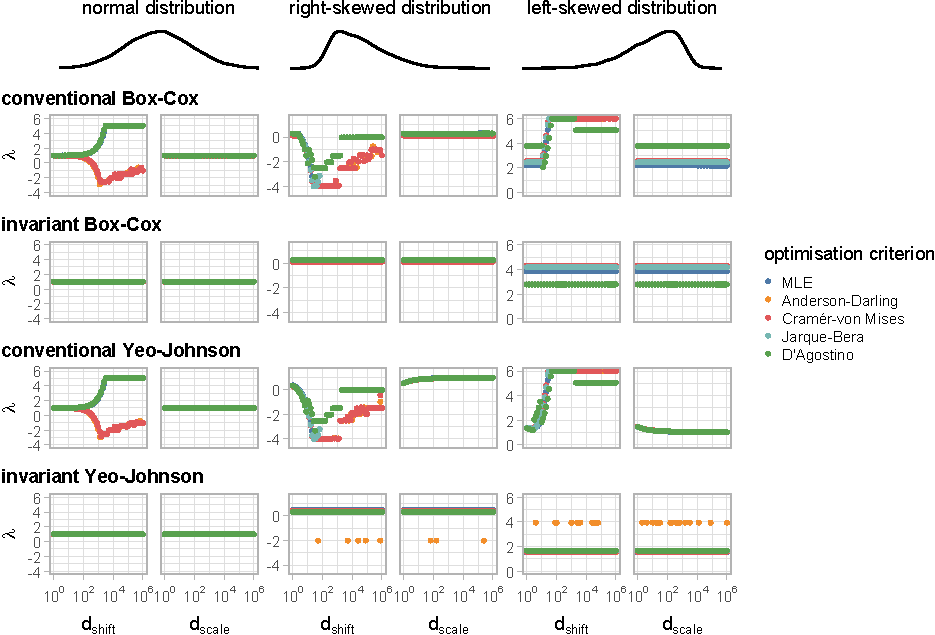
\includegraphics[width=1\linewidth]{figure_appendix_1} 

}

\caption{Invariant power transformation produces transformation parameters that are invariant to location and scale. Samples were drawn from normal, right-skewed and left-skewed distributions, respectively, which then underwent a shift $d_{\text{shift}}$ or multiplication by $d_{\text{scale}}$. Estimates of the transformation parameter $\lambda$ for the conventional power transformations show strong dependency on the overall location and scale of the distribution and the optimisation criterion, whereas estimates obtained for the location- and scale-invariant power transformations are constant. For location- and scale-invariant power transformations, the Anderson-Darling criterion leads to unstable estimates of $\lambda$ for skewed distributions, possibly due to large weights being assigned to samples at the upper and lower ends of the distribution.}\label{fig:shifted-distributions-appendix}
\end{figure}

\section{Experimental results using location- and scale-invariant Box-Cox transformation}
\label{appendix-d-experimental-results-using-location--and-scale-invariant-box-cox-transformation}

The effect of using location- and scale-invariant transformations was
investigated using real-world datasets.

\subsection{Invariance}\label{sec-app:invariance}

Results for Box-Cox transformations of features without outliers are
shown in Figure \ref{fig:experimental-results-invariance-appendix}.

\begin{figure}

{\centering 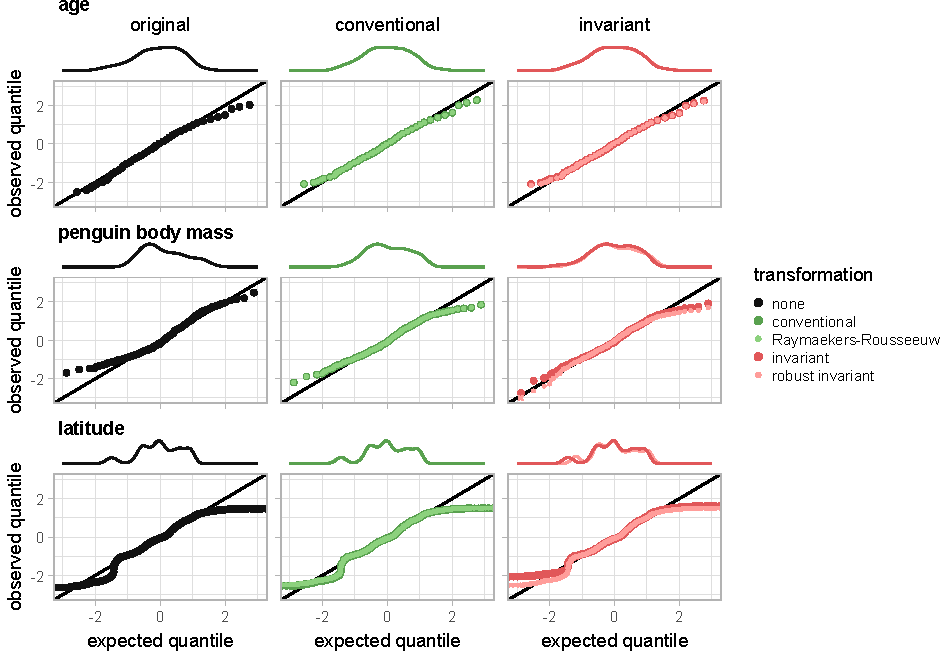
\includegraphics[width=1\linewidth]{figure_appendix_2} 

}

\caption{Quantile-quantile plots for several datasets: age of patients with lung cancer (top row); penguin body mass (middle row); and latitude coordinates of houses sold in Ames, Iowa (bottom row). Multiple quantile-quantile plots are shown: for the original feature (left column); the feature transformed using the conventional Box-Cox transformation and Raymaekers and Rousseeuw's robust adaptation (middle column); and the feature transformed using the non-robust and robust location- and-scale invariant Box-Cox transformations (right column).}\label{fig:experimental-results-invariance-appendix}
\end{figure}

\subsubsection{Age of patients with lung
cancer}\label{sec-app:age-of-patients-with-lung-cancer}

Applying conventional and invariant Box-Cox transformations to age of
patients with lung cancer \citep{Loprinzi1994-cd} yielded the following
results: no transformation (sum of residuals with normal distribution
\(\sum r_i = 16.5\)); conventional transformation (\(\lambda = 1.9\),
\(\sum r_i = 11.5\), \(\mu_{BC} = 1.6 \cdot 10^3\),
\(\sigma_{BC} = 0.4 \cdot 10^3\)); Raymaekers and Rousseeuw's robust
adaptation (\(\lambda = 1.9\), \(\sum r_i = 11.5\),
\(\mu_{BC} = 1.6 \cdot 10^3\), \(\sigma_{BC} = 0.4 \cdot 10^3\));
location- and scale-invariant transformation (\(\lambda = 1.7\),
\(\sum r_i = 11.6\), \(\mu_{BC} = 1.9\), \(\sigma_{BC} = 0.8\)); and
robust location- and scale-invariant transformation (\(\lambda = 1.5\),
\(\sum r_i = 11.6\), \(\mu_{BC} = 3.6\), \(\sigma_{BC} = 1.2\)).

Compared to location- and scale-invariant Yeo-Johnson transformations,
the Box-Cox transformations do not reduce residuals compared to
conventional variants.

\subsubsection{Penguin body mass}\label{sec-app:penguin-body-mass}

Applying conventional and invariant Box-Cox transformations to the body
mass of penguins \citep{Gorman2014-eo} yielded the
following results: no transformation (residual sum \(\sum r_i = 48.0\));
conventional transformation (\(\lambda = -0.5\), \(\sum r_i = 32.2\),
\(\mu_{BC} = 2.1\), \(\sigma_{BC} = 4 \cdot 10^{-3}\)); Raymaekers and
Rousseeuw's robust adaptation (\(\lambda = -0.5\), \(\sum r_i = 32.2\),
\(\mu_{BC} = 2.1\), \(\sigma_{BC} = 4 \cdot 10^{-3}\)); location- and
scale-invariant transformation (\(\lambda = 0.5\), \(\sum r_i = 27.3\),
\(\mu_{BC} = 0.3\), \(\sigma_{BC} = 0.6\)); and robust location- and
scale-invariant transformation (\(\lambda = 0.2\), \(\sum r_i = 25.2\),
\(\mu_{BC} = 0.4\), \(\sigma_{BC} = 0.6\)).

Just as for location- and scale-invariant Yeo-Johnson transformations,
Box-Cox transformations produced a lower overall residual sum compared
to their conventional counterparts. Similarly, conventional
transformations led to low standard deviation \(\sigma_{YJ}\) of the
body mass feature after transformation.

\subsubsection{Latitude in the Ames housing
dataset}\label{sec-app:latitude-in-the-ames-housing-dataset}

Applying conventional and invariant Box-Cox transformations to the
latitude of houses in the Ames housing dataset \citep{De-Cock2011-jf} yielded
the following results: no transformation (residual sum
\(\sum r_i = 328\)); conventional transformation (\(\lambda = 62.1\),
\(\sum r_i = 319\), \(\mu_{BC} = 1.1 \cdot 10^{99}\),
\(\sigma_{BC} = 0.0 \cdot 10^{99}\)); Raymaekers and Rousseeuw's robust
adaptation (\(\lambda = 96.0\), \(\sum r_i = 319\),
\(\mu_{BC} = 6.2 \cdot 10^{153}\),
\(\sigma_{BC} = 0.3 \cdot 10^{153}\)); location- and scale-invariant
transformation (\(\lambda = 1.9\), \(\sum r_i = 312\),
\(\mu_{BC} = 2.3\), \(\sigma_{BC} = 0.9\)); and robust location- and
scale-invariant transformation (\(\lambda = 1.2\), \(\sum r_i = 316\),
\(\mu_{BC} = 5.5\), \(\sigma_{BC} = 1.4\)).

Similar to conventional Yeo-Johnson transformations (non-robust and
robust), conventional Box-Cox transformations had high values for the
\(\lambda\) parameter, which could lead to numerical issues. Location-
and scale-invariant Box-Cox transformations did not suffer from this
issue.

\subsection{Robustness against
outliers}\label{sec-app:robustness-against-outliers}

Results for Box-Cox transformations of features with outliers are shown
in Figure \ref{fig:experimental-results-outlier-robustness-appendix}.

\begin{figure}

{\centering 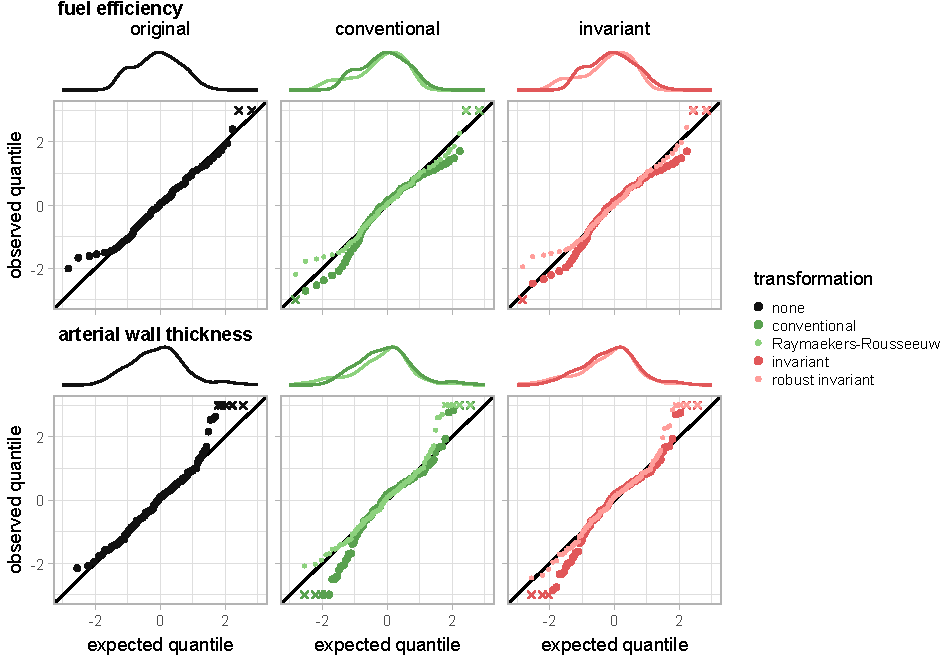
\includegraphics[width=1\linewidth]{figure_appendix_3} 

}

\caption{Quantile-quantile plots for two datasets with outliers: vehicle fuel consumption (top row), where outliers are related to highly fuel-efficient vehicles; and maximum arterial wall thickness in patients with ischemic stroke (bottom row). Multiple quantile-quantile plots are shown: for the original feature (left column); the feature transformed using the conventional Box-Cox transformation and Raymaekers and Rousseeuw's robust adaptation (middle column); and the feature transformed using the non-robust and robust location- and-scale invariant Box-Cox transformations (right column). Samples with observed quantiles below $-3.0$ or above $3.0$ are indicated by crosses.}\label{fig:experimental-results-outlier-robustness-appendix}
\end{figure}

\subsubsection{Fuel efficiency in the Top Gear
dataset}\label{sec-app:fuel-efficiency-in-the-top-gear-dataset}

The Top Gear dataset contains data on 297 vehicles, with outliers
related highly fuel-efficient vehicles \citep{Alfons2021-kc}. Applying
conventional and invariant Box-Cox transformations to the fuel
consumption feature yielded the following results: no transformation
(residual sum \(\sum r_i = 54\), \(p=0.76\)); conventional
transformation (\(\lambda = -0.1\), \(\sum r_i = 55\),
\(\mu_{BC} = 3.0\), \(\sigma_{BC} = 0.3\), \(p=0.01\)); Raymaekers and
Rousseeuw's robust adaptation (\(\lambda = 0.8\), \(\sum r_i = 48\),
\(\mu_{BC} = 29\), \(\sigma_{BC} = 15\), \(p=0.55\)); location- and
scale-invariant transformation (\(\lambda = -0.7\), \(\sum r_i = 44\),
\(\mu_{BC} = 0.6\), \(\sigma_{BC} = 0.2\), \(p=0.02\)); and robust
location- and scale-invariant transformation (\(\lambda = 1.1\),
\(\sum r_i = 59\), \(\mu_{BC} = 2.4\), \(\sigma_{BC} = 1.8\),
\(p=0.83\)).

\subsubsection{Maximum arterial wall thickness in an ischemic stroke
dataset}\label{sec-app:maximum-arterial-wall-thickness-in-an-ischemic-stroke-dataset}

The ischemic stroke dataset contains historic data from 126 patients
with risk at ischemic stroke \citep{Kuhn2019-kt}. Applying
conventional and invariant Box-Cox transformations to the maximum
arterial wall thickness feature yielded the following results: no
transformation (residual sum \(\sum r_i = 110\), \(p=0.56\));
conventional transformation (\(\lambda = -0.5\), \(\sum r_i = 33\),
\(\mu_{BC} = 1.0\), \(\sigma_{BC} = 0.2\), \(p=0.01\)); Raymaekers and
Rousseeuw's robust adaptation (\(\lambda = 1.1\), \(\sum r_i = 127\),
\(\mu_{BC} = 5.5\), \(\sigma_{BC} = 12\), \(p=0.60\)); location- and
scale-invariant transformation (\(\lambda = -1.0\), \(\sum r_i = 28\),
\(\mu_{BC} = 0.7\), \(\sigma_{BC} = 0.1\), \(p=0.01\)); and robust
location- and scale-invariant transformation (\(\lambda = 0.5\),
\(\sum r_i = 56\), \(\mu_{BC} = 2.2\), \(\sigma_{BC} = 1.4\),
\(p=0.35\)).

\section{Empirical central normality test}\label{appendix-e-empirical-central-normality-test}

The empirical central normality test was derived using data sampled from
asymmetric generalised normal distributions, including outliers, to
resemble more realistic datasets. Here we assess the type I error rate
of two, less realistic, sets of data:

\begin{enumerate}
\def\labelenumi{\arabic{enumi}.}
\item
  Data sampled from asymmetric generalised normal distributions without
  outliers.
\item
  Data sampled from normal distributions without outliers, without any
  power transformation applied.
\end{enumerate}

Other aspects of the experiment remained the same. Thus, we first drew
\(m_d=10000\) random distributions. For asymmetric generalised normal
distributions, each distribution was parametrised with a randomly chosen
skewness parameter \(\alpha \sim U\left(0.01, 0.99\right)\) and shape
parameter \(\beta \sim U\left(1.00, 5.00 \right)\). For fully normal
distributions, skewness parameter \(\alpha = 0.5\) and shape parameter
\(\beta = 2.0\) were fixed. Location and scale parameters were set as
\(\mu = 0\) and \(\sigma = 1\), respectively.
\(n = \lceil 10^\gamma \rceil\) values were then randomly drawn, with
\(\gamma \sim U\left(1.47, 3.00\right)\), which led to between \(30\)
and \(1000\) values being drawn to create \(\mathbf{X}_i\). Residuals
were then computed after performing robust location- and scale-invariant
transformations with the empirical tapered cosine weighting method for
the dataset with asymmetric generalised normal distributions, and
without any transformation for the dataset with only normal
distributions.

\begin{figure}

{\centering 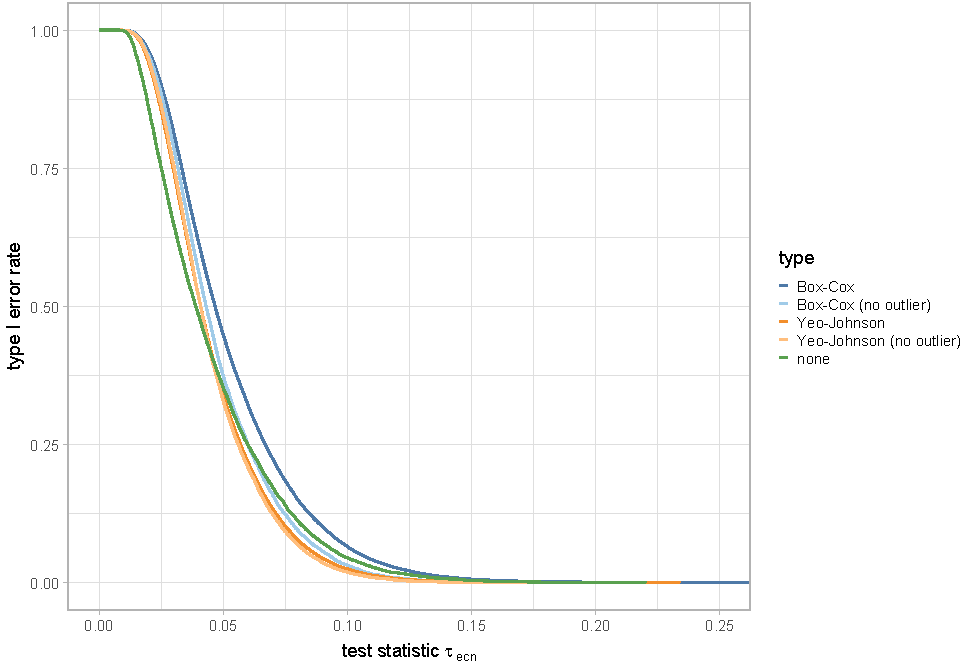
\includegraphics[width=1\linewidth]{figure_appendix_4} 

}

\caption{Type I error rate as function of the test statistic $\tau_{\text{ecn}}$ for five datasets, with central portion $\kappa=0.80$. The type I error rate is computed from $m_d=10000$ randomly sampled features, These are sampled from asymmetric generalized normal distributions, with and without outliers (Box-Cox and Yeo-Johnson), or normal distributions with outliers (none). The test statistic is computed as the average residual of each feature after (Box-Cox and Yeo-Johnson) robust location- and shift-invariant power transformation, or before (none).}\label{fig:empirical-central-normality-test-appendix}
\end{figure}

\begin{table}
\begin{center}
\caption{Test statistic $\tau_{\text{ecn}}$ for empirical central normality at $\kappa = 0.80$ as a function of Type I error rate for several datasets.}
\label{tab:empirical-central-normality-appendix}
\begin{tabular}{l | c c c c c c c}

\toprule
type I error rate & 0.50 & 0.20 & 0.10 & 0.05 & 0.02 & 0.01 & 0.001 \\

\midrule
Box-Cox                  & 0.047 & 0.073 & 0.090 & 0.106 & 0.126 & 0.140 & 0.188 \\
Box-Cox (no outlier)     & 0.043 & 0.065 & 0.079 & 0.092 & 0.106 & 0.116 & 0.155 \\
Yeo-Johnson              & 0.041 & 0.062 & 0.075 & 0.088 & 0.103 & 0.115 & 0.154 \\
Yeo-Johnson (no outlier) & 0.041 & 0.061 & 0.074 & 0.085 & 0.099 & 0.109 & 0.139 \\
normal distr.            & 0.039 & 0.066 & 0.083 & 0.097 & 0.117 & 0.132 & 0.174 \\
\bottomrule

\end{tabular}
\end{center}
\end{table}

The results are shown in Figure
\ref{fig:empirical-central-normality-test-appendix} and Table
\ref {tab:empirical-central-normality-appendix}. These indicate that the
test behaves similarly for the different datasets. For low type I error
rates, the test statistic proposed in section \ref{empirical-central-normality-test-1} is more
conservative than alternatives based on residuals after Box-Cox
transformations of asymmetric generalised normally distributed features
or on residuals from strictly normally distributed features.

\section{Normalisation before transformation}\label{appendix-f-normalisation-before-transformation}

An alternative to location- and scale-invariant transformations is
normalising feature distributions prior to conventional transformations.
Table \ref{tab:normalisation-before-transformation-appendix} shows
residual errors, after transformation to normality, of the five features
from real-world datasets presented previously section \ref{experimental-results}
and \ref{appendix-d-experimental-results-using-location--and-scale-invariant-box-cox-transformation}.
In these examples location- and scale-invariant
transformations have similar or lower residual errors compared to errors
resulting from normalisation prior to transformation.

\begin{table}
\begin{center}
\caption{Residual errors for features from real-world datasets after Yeo-Johnson transformation to normality. conv.: conventional; norm.: normalisation; rob.: robust}
\label{tab:normalisation-before-transformation-appendix}
\begin{tabular}{l | c c c c c}

\toprule
feature & none & conv. & conv. (z-score norm.) & conv. (rob. scaling) & invariant \\

\midrule
age                     &  16.5 &  11.5 &  11.5 &  11.3 &   8.8 \\
penguin body mass       &  48.0 &  32.2 &  33.3 &  32.2 &  26.8 \\
latitude                & 328.1 & 319.0 & 326.2 & 324.5 & 326.4 \\
fuel efficiency         &  54.5 &  55.3 &  49.0 &  53.3 &  44.0 \\
arterial wall thickness & 110.1 &  30.0 &  19.3 &  31.8 &  12.2 \\
\bottomrule
\end{tabular}
\end{center}
\end{table}

%% For citations use:
%%       \citet{<label>} ==> Lamport (1994)
%%       \citep{<label>} ==> (Lamport, 1994)
%%
%% Example citation, See \citet{lamport94}.

%% If you have bib database file and want bibtex to generate the
%% bibitems, please use
%%
%%  \bibliographystyle{elsarticle-harv}
%%  \bibliography{<your bibdatabase>}

\bibliographystyle{elsarticle-harv}
\bibliography{refs}

\end{document}

\endinput
%%
%% End of file `elsarticle-template-harv.tex'.


